\chapter{Null geodesics and images in Schwarzschild spacetime}
\label{s:gis}

\minitoc

\section{Introduction}

Having investigated the properties of generic causal geodesics
in Schwarzschild spacetime in Chap.~\ref{s:ges}, we focus here on null
geodesics.


%%%%%%%%%%%%%%%%%%%%%%%%%%%%%%%%%%%%%%%%%%%%%%%%%%%%%%%%%%%%%%%%%%%%%%%%%%%%%%%

\section{Main properties of null geodesics} \label{s:ges:null}

We use the same notations as in Sec.~\ref{s:ges:geod_motion} of the preceding
chapter: $(\M, \w{g})$ is Schwarzschild spacetime, $(t,r,\th,\ph)$ are
Schwarzschild-Droste coordinates and
$\mathscr{P}$ is a particle, the worldline of which is a
geodesic $\Li$. The particle $\mathscr{P}$ is characterized by its
4-momentum $\w{p}$ and
$E$ and $L$ are respectively the conserved energy and conserved angular momentum
along $\Li$ [cf.~Eq.~(\ref{e:ges:conserved_quantities})].


In all this chapter, we consider that $\Li$ is a null geodesic, or equivalently that
$\mathscr{P}$ is a massless particle, typically a photon\index{photon}.
As in Chap.~\ref{s:ges}, we assume that the coordinates $(\th,\ph)$ are chosen
so that $\Li$ lies in the hyperplane $\th=\pi/2$. Let us recall that
a geodesic of Schwarzschild spacetime lies necessarily in some hypersurface, which
can be chosen to be the hyperplane $\th=\pi/2$ without any loss of generality
(cf. Sec.~\ref{s:ges:fiom}).

\subsection{Equation to be solved}

In terms of Schwarzschild-Droste coordinates, the motion of $\mathscr{P}$ is governed by Eqs.~(\ref{e:ges:dot_t}), (\ref{e:ges:dot_ph}) and (\ref{e:ges:dot_r_square})
with $\mu=0$ (massless particle):
\be \label{e:ges:dot_t_null}
   \encadre{ \frac{\D t}{\D \lambda} = E \left(1 - \frac{2m}{r} \right) ^{-1} } ,
\ee
\be \label{e:ges:dot_ph_null}
   \encadre{ \frac{\D\ph}{\D\lambda} = \frac{L}{r^2}  },
\ee
\be \label{e:ges:dot_r_square_null}
   \encadre{ \left( \frac{\D r}{\D \lambda} \right) ^2
         + \frac{L^2}{r^2}
         \left( 1 - \frac{2m}{r} \right) = E^2 }.
\ee
Let us recall that the variable $\lambda$ with respect to which these differential equations
hold
is the affine parameter associated with the 4-momentum $\w{p}$ of $\mathscr{P}$
(cf. Eq.~(\ref{e:ges:def_lambda})) and that it increases towards the future,
$\w{p}$ being future-oriented (cf. Sec.~\ref{s:ges:eq_to_be_solved}).

\subsection{Radial null geodesics} \label{s:gis:radial}

Let us first discuss the case of a radial geodesic: $L=0$.
Equation (\ref{e:ges:dot_ph_null}) yields then naturally $\ph=\mathrm{const}$,
while Eq.~(\ref{e:ges:dot_r_square_null}) simplifies drastically:
\be \label{e:ges:dot_r_null_radial}
    \frac{\D r}{\D \lambda} = \pm E ,
\ee
the solution of which is immediate:
\be \label{e:ges:r_lambda_radial_null}
    r = \pm E\lambda + r_0 ,
\ee
where $r_0$ is some constant.
Moreover, writing $\D t/\D\lambda = \D t/\D r \times \D r/\D\lambda$
and combining Eqs.~(\ref{e:ges:dot_t_null}) and (\ref{e:ges:dot_r_null_radial}),
we get
\be
    \frac{\D t}{\D r} = \pm \left(1 - \frac{2m}{r} \right) ^{-1} .
\ee
We recognize the equation governing the radial null geodesics obtained in
Sec.~\ref{s:sch:rad_null_geod} [Eq.~(\ref{e:sch:Dt_Dr_radial_null_geod})],
the solution of which is given by Eq.~(\ref{e:sch:t_r_radial_null_geod}):
\be
   \encadre{ t = \pm r \pm 2 m \ln \left| \frac{r}{2m} - 1 \right| + \mathrm{const} }.
\ee

\begin{remark}
Since $\lambda$ is an affine parameter and $E$ is constant,
Eq.~(\ref{e:ges:r_lambda_radial_null})
shows explicitly that $r$ is another affine parameter along the radial null
geodesics of Schwarzschild spacetime --- a result that we had already
obtained in Sec.~\ref{s:sch:rad_null_geod}.
\end{remark}

The radial null geodesics of Schwarzschild spacetime are plotted in
Fig.~\ref{f:sch:rad_null_geod} in terms of the Schwarzschild-Droste coordinates
and in Fig.~\ref{f:sch:rad_null_geod_EF} in terms of the ingoing Eddington-Finkelstein coordinates.



\subsection{Generic null geodesics: effective potential}
\label{s:ges:null_eff_pot}

Here we focus on the case where $L\not= 0$ (``generic'' case). We may then
consider, instead of $\lambda$, the affine parameter
\be
    \tilde{\lambda} := |L| \lambda .
\ee
Since $L$ is a non-vanishing constant along a geodesic, the above formula
does define a new affine parameter. The absolute value ensures that
$\tilde{\lambda}$ is increasing towards the future, as $\lambda$, whatever
the sign of $L$. Note that $\tilde{\lambda}$ has the same
dimension as $L$, i.e. a squared length, given that $\lambda$ is dimensionless
(cf. Sec.~\ref{s:ges:eq_to_be_solved}).
In terms of $\tilde{\lambda}$,
the differential system (\ref{e:ges:dot_t_null})-(\ref{e:ges:dot_r_square_null})
becomes
\be \label{e:ges:dot_t_null_b}
   \encadre{\frac{\D t}{\D \tilde{\lambda}} = b^{-1} \left(1 - \frac{2m}{r} \right) ^{-1} },
\ee
\be \label{e:ges:dot_ph_null_b}
   \encadre{ \frac{\D\ph}{\D\tilde{\lambda}} = \frac{\epsilon_L}{r^2} } ,
\ee
\be \label{e:ges:dot_r_square_null_b}
   \encadre{ \left( \frac{\D r}{\D\tilde{\lambda}} \right) ^2
        + U(r) = \frac{1}{b^2} },
\ee
where
\be \label{e:ges:def_b}
    \encadre{b := \frac{|L|}{E}} ,
\ee
\be \label{e:gis:def_epsilon_L}
    \epsilon_L := \frac{L}{|L|} = \operatorname{sgn} L
\ee
and
\be \label{e:ges:eff_pot_null}
    \encadre{ U(r) := \frac{1}{r^2} \left( 1 - \frac{2m}{r} \right) }.
\ee
As for the timelike case (cf. Eq.~(\ref{e:ges:1d_motion_timelike})),
we note that Eq.~(\ref{e:ges:dot_r_square_null_b})
has the shape of the first integral of the
1-dimensional motion of a non-relativist particle in the
\defin{effective potential}\index{effective!potential!null geodesic}
$U(r)$. The main difference is that $U(r)$ does not depend on $L$, contrary
to the effective potential $V_\ell(r)$ for timelike geodesics. Actually,
$U(r)$ is a function of $r$ and the black hole mass $m$ only.
Null geodesics are thus entirely determined by the parameter
$b$ and $\epsilon_L = \pm 1$.
As soon as the null geodesic $\Li$ has a part in the
region $\M_{\rm I}$, then $E>0$ [cf. (\ref{e:ges:E_positive_M_I})], so that
$b$, as defined by Eq.~(\ref{e:ges:def_b}), is finite and positive. It has
has the dimension of a length
and can be interpreted as the
\defin{impact parameter}\index{impact parameter} in the case of a
particle arising from infinity.
\begin{proof}
Let us consider that the massless
particle $\mathscr{P}$ arises from a point of coordinates $\theta=\pi/2$,
$r=r_0 \gg m$ and $\ph = \ph_0$.  Let us introduce
Cartesian coordinates $(x,y)$ in the plane $\theta=\pi/2$:
$x:=r\cos\ph$ and $y:=r\sin\ph$.
Without any loss of generality, we may
consider $|\ph_0| \ll 1$. For large values of $r$, the motion of
$\mathscr{P}$ is then essentially along the $x$-axis, with $\ph$ remaining small:
$y\simeq y_0$, where
$y_0 = r_0 \sin\ph_0 \simeq r_0 \ph_0$. The quantity
$|y_0|$ is the impact parameter.
Since $y=r\sin\ph\simeq r\ph$, we get from $y\simeq y_0$
the following relation
\[
    \ph \simeq \frac{y_0}{r} \qquad (r \gg m) .
\]
Deriving with respect to $t$ leads to
\be \label{e:ges:dphdt_approx}
    \derd{\ph}{t} \simeq - \frac{y_0}{r^2} \derd{r}{t}
                  \simeq \frac{y_0}{r^2}  \qquad (r \gg m) ,
\ee
where we have used $\D r / \D t = - 1$ for $r \gg m$. This last property is easy
to admit since
$r\gg m$ corresponds to the flat part of spacetime; however, it can be derived
rigorously by combining Eqs.~(\ref{e:ges:dot_t_null_b}) and
(\ref{e:ges:dot_r_square_null_b}) to evaluate $\D r / \D t$.
Now by combining Eqs.~(\ref{e:ges:dot_t_null_b}) and (\ref{e:ges:dot_ph_null_b}),
we have
\be
    \derd{\ph}{t} = \epsilon_L \frac{b}{r^2} \left( 1 - \frac{2m}{r} \right) .
\ee
For $r\gg m$, the right-hand side reduces to $\epsilon_L b/r^2$, so that the comparison
with (\ref{e:ges:dphdt_approx}) yields $\epsilon_L b = y_0$, i.e. $b = |y_0|$,
which proves that $b$ is the impact
parameter of the massless particle $\mathscr{P}$ with respect to the central
black hole.
\end{proof}

\begin{figure}
\centerline{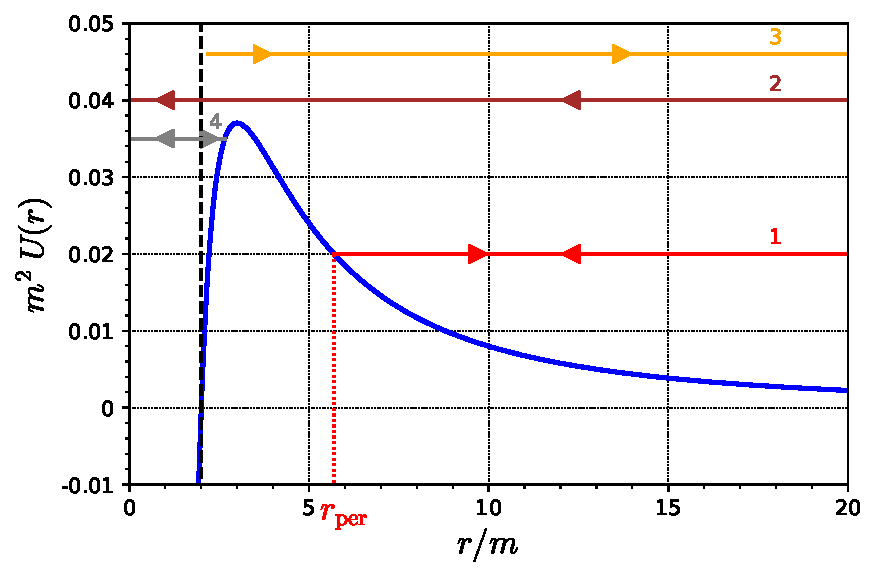
\includegraphics[width=0.8\textwidth]{ges_eff_pot_null.pdf}}
\caption[]{\label{f:gis:eff_pot_null} \footnotesize
Effective potential $U(r)$ (rescaled by $m^2$ to make it dimensionless)
governing the $r$-part of the
motion along a null geodesic in
Schwarzschild spacetime [Eq.~(\ref{e:ges:eff_pot_null})].
The vertical dashed line marks $r=2m$, i.e. the
location of the event horizon. The horizontal lines marked ``1'' to ``4''
correspond to the $r$-motion of four null geodesics,
the trajectories of which in the equatorial plane $\th=\pi/2$
are depicted in Fig.~\ref{f:gis:null_geod}.}
\end{figure}

\begin{figure}
\centerline{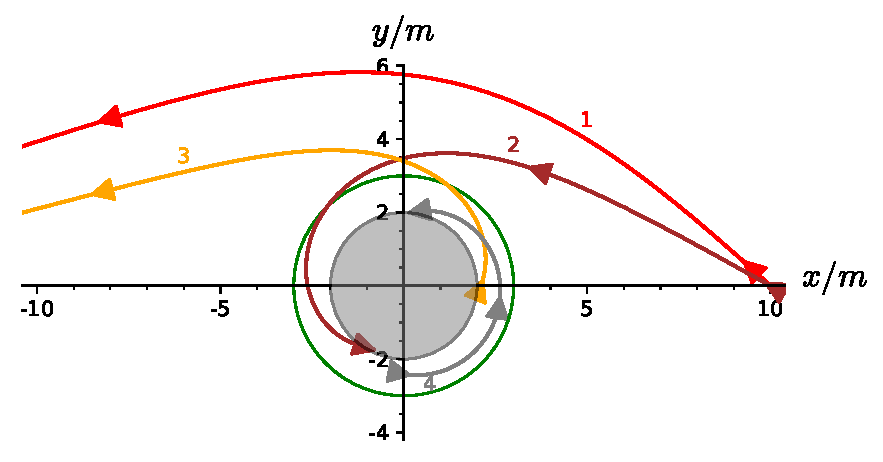
\includegraphics[width=0.8\textwidth]{ges_null_geod.pdf}}
\caption[]{\label{f:gis:null_geod} \footnotesize
Selected null geodesics in the equatorial plane of Schwarzschild spacetime,
plotted in terms
of the coordinates $(x,y) := (r\cos\ph, r\sin\ph)$, with the black hole
region $r<2m$ depicted as a grey disk.
The green geodesic is the photon circular orbit at $r=3m$.
The red geodesic (label ``1'') starts at $r_0=10 m$, $\ph_0=0$, with
the impact parameter $b = 7.071 \, m > b_{\rm c}$ ($b^{-2} = 0.02\, m^{-2}$).
The brown geodesic (label ``2'') starts at $r_0=10 m$, $\ph_0=0$ with $b = 5 m < b_{\rm c}$ ($b^{-2} = 0.04\, m^{-2}$).
The orange geodesic (label ``3'') starts outward at $r_0=2.1 m$, $\ph_0=0$ with $b = 4.663 m$ ($b^{-2} = 0.046\, m^{-2}$).
The grey geodesic (label ``4'') starts outward at $r_0=2.4 m$, $\ph_0=-\pi/2$ with $b = 5.345 m$ ($b^{-2} = 0.035\, m^{-2}$).
The $r$-motion of these four gedeosics is depicted in
Fig.~\ref{f:gis:eff_pot_null}.}
\end{figure}

The effective potential $U(r)$ is plotted in Fig.~\ref{f:gis:eff_pot_null}.
It has no minimum and a maximum at $r=3m$, which is
\be \label{e:ges:U_max}
    U_{\rm max} = \frac{1}{27m^2} .
\ee
This extremum is a stationary position in $r$: it corresponds thus to a circular
orbit, usually called the \defin{photon orbit}\index{photon!orbit}\index{orbit!photon --}.
The set of all photon orbits (one per choice of equatorial plane) is often
called the \defin{photon sphere}\index{photon!sphere}\index{sphere!photon --}.
However, since it corresponds to a \emph{maximum} of the effective potential, the circular
orbit at $r=3m$ is an unstable orbit. So one should not imagine that a
Schwarzschild black hole is surrounded by any spherical shell of photons...


\subsection{Radial behaviour of null geodesics} \label{s:ges:null_radial_behav}

For the sake of concreteness, in this section and the remaining ones, we
refer to the massless particle $\mathscr{P}$ as a ``photon''. In most applications, in
particular the astrophysical ones, $\mathscr{P}$ will indeed be a photon.
But one shall keep in mind that all results are valid for any other massless
particle.

Since the effective potential
$U(r)$ has no minimum, it does not offer any potential well,
as it is clear from Fig.~\ref{f:gis:eff_pot_null}. This is in sharp contrast
with the effective potential $V_\ell(r)$ for massive particle
(compare Fig.~\ref{f:ges:eff_pot_bound}). Hence there are no bound orbits
for photons\footnote{unless one counts as ``bound'' a worldline that terminates in the
black hole region}.

We can infer various types of photon worldlines from Fig.~\ref{f:gis:eff_pot_null}.
In view of the ``first integral'' (\ref{e:ges:dot_r_square_null_b}),
each photon worldline can be represented by a horizontal line of ordinate
$b^{-2}$ in this figure, which must lie above the curve $U(r)$
by the positive quantity $({\D r}/{\D\tilde{\lambda}})^2$. The region under the curve
$U(r)$ is thus excluded.

For an initially inward photon, i.e. a photon emitted with ${\D r}/{\D\tilde{\lambda}} < 0$
from a position $r=r_{\rm em}$, there are
two possibilities, depending on the values of $r_{\rm em}$ and
of the impact parameter $b$:
\begin{itemize}
\item if $r_{\rm em} > 3 m$ and $b$ is large enough to fulfil $b^{-2} < U_{\rm max}$
(e.g. trajectory no.~1 in Fig.~\ref{f:gis:eff_pot_null}), the photon
``bounces'' on the potential barrier constituted by $U(r)$
at some minimal value  $r_{\rm p}$ of $r$ --- the \defin{periastron}\index{periastron},
which is given by  $U(r_{\rm p}) = b^{-2}$, or equivalently by
\be \label{e:ges:r_per_null}
  r_{\rm p}^3 - b^2\, r_{\rm p} + 2 m b^2 = 0, \quad r_{\rm p} > 3 m.
\ee
Equation~(\ref{e:ges:dot_r_square_null_b})
implies then
\be
    \left. \frac{\D r}{\D\tilde{\lambda}} \right| _{r = r_{\rm p}} = 0 .
\ee
Actually, $\D r / \D\tilde{\lambda}$ changes sign at $r = r_{\rm p}$ and
the photon subsequently moves away from the black hole for ever (cf. geodesic
no.~1 in Fig.~\ref{f:gis:null_geod}). We may call
such a worldline a scattering trajectory.
\item if $r_{\rm em} < 3 m$ (e.g. trajectory
no.~4 in Fig.~\ref{f:gis:eff_pot_null}) or $b$ is small enough to fulfil $b^{-2} > U_{\rm max}$ ((e.g. trajectory
no.~2 in Fig.~\ref{f:gis:eff_pot_null}) the photon
is not halted by the potential barrier constituted by $U(r)$. It then reaches arbitrary
small values of $r$ and is eventually absorbed by the black hole ($r < 2m$)
(cf. geodesic no.~2 in Fig.~\ref{f:gis:null_geod}).
\end{itemize}

For an initially outward photon, i.e. a photon emitted with ${\D r}/{\D\tilde{\lambda}} > 0$,
one has necessarily $r_{\rm em}>2m$ according to the result obtained in Sec.~\ref{s:ges:eq_to_be_solved}
and there are then two possible outcomes:

\begin{itemize}
\item if $r_{\rm em} > 3 m$ (e.g. trajectory
no.~1 in Fig.~\ref{f:gis:eff_pot_null}) or
$b$ is small enough to fulfil $b^{-2} > U_{\rm max}$ (e.g. trajectory
no.~3 in Figs.~\ref{f:gis:eff_pot_null}), the photon escapes to infinity
(cf. geodesic no.~3 in Fig.~\ref{f:gis:null_geod});
\item if $2m < r_{\rm em} < 3 m$ and $b^{-2} < U_{\rm max}$ (e.g. trajectory
no.~4 in Fig.~\ref{f:gis:eff_pot_null}), the photon ``bounces'' on the left
side of the potential barrier, reaching a maximal value $r_{\rm a}$ of $r$
--- the \defin{apoastron}\index{apoastron},
which is given by  $U(r_{\rm a}) = b^{-2}$, or equivalently by
\be \label{e:ges:r_apo_null}
   r_{\rm a}^3 - b^2\, r_{\rm a} + 2 m b^2 = 0, \quad r_{\rm a} < 3 m.
\ee
The photon moves subsequently towards the black hole and
is absorbed by it (cf. geodesic no.~4 in Fig.~\ref{f:gis:null_geod}).
\end{itemize}

The critical value of the impact parameter $b$ separating the cases discussed
above is determined by $b_{\rm c}^{-2} = U_{\rm max}$.
Given the value (\ref{e:ges:U_max}) of $U_{\rm max}$, we get
\be \label{e:ges:b_crit}
    \encadre{b_{\rm c} = 3\sqrt{3} \, m \simeq 5.196152\, m }.
\ee

It follows from the above discussion that
\begin{greybox}
Along any null geodesic of Schwarzschild spacetime, the areal coordinate $r$
either is a monotonic function or has a single turning point. In the latter case,
if the turning point corresponds to a minimum of $r$ (a periastron, which can occur
only for $r>3m$), the null geodesic escapes to infinity, while if the turning
point corresponds to a maximum of $r$ (an apoastron, which can occur only for $2m<r<3m$), the
null geodesic terminates at the central singularity ($r=0$).
\end{greybox}
Note that for $r<2m$, i.e. in the black hole region, $r$
is always a monotonic function, since it has been demonstrated in
Sec.~\ref{s:ges:eq_to_be_solved} that $r(\lambda)$ is strictly
decreasing. The impossibility of a turning point for $r<2m$ can also be
graphically inferred from Fig.~\ref{f:gis:eff_pot_null}, which shows
that the effective potential $U(r)$ is negative for $r<2m$,
preventing the turning point condition $U(r) = b^{-2}$ to hold.


For $b > b_{\rm c}$, the explicit expression of the periastron radius
$r_{\rm p}$ (or the apoastron radius $r_{\rm a}$)
is obtained by solving the cubic equation (\ref{e:ges:r_per_null})
(or (\ref{e:ges:r_apo_null}), which is the same cubic equation, except for
the range of the solution). Fortunately Eq.~(\ref{e:ges:r_per_null})
is a depressed\footnote{A \emph{depressed} cubic equation is a polynomial equation
of the type $x^3 + p x + q = 0$.} cubic equation, which makes
it simpler to solve. For $b > b_{\rm c}$, its discriminant is positive, which
implies that it admits three distinct real roots. Two of them are positive
and are precisely $r_{\rm p}$ and $r_{\rm a}$. The third root is negative,
since the product of the roots is $-2mb^2 < 0$; it has therefore no
physical significance. The roots of the generic depressed cubic
equation $x^3 + p x + q = 0$ can be expressed via Viète's formulas:
\be \label{e:gis:Viete}
    x_k = 2 \sqrt{-\frac{p}{3}} \cos \left[ \frac{1}{3}\,  \arccos\left(
        \frac{3 q}{2 p} \sqrt{-\frac{3}{p}} \right) + \frac{2 k\pi}{3} \right],
        \qquad k \in \{0, 1, 2\} .
\ee
In the present case, $p= - b^2$ and $q = 2 m b^2$,
and $r_{\rm p}$ (resp. $r_{\rm a}$) corresponds to $k=0$
(resp. $k=2$), so that we obtain
\be \label{e:ges:sol_r_per}
  \encadre{  r_{\rm p} = \frac{2 b}{\sqrt{3}} \cos\left[\frac{\pi}{3}
        - \frac{1}{3} \, \arccos\left(\frac{b_{\rm c}}{b}\right) \right] }.
\ee
\be \label{e:ges:sol_r_apo}
   \encadre{ r_{\rm a} = \frac{2 b}{\sqrt{3}} \cos\left[\frac{5\pi}{3}
        - \frac{1}{3} \, \arccos\left(\frac{b_{\rm c}}{b}\right) \right] }.
\ee
As a check, we note that for $b\gg b_{\rm c}$, Eq.~(\ref{e:ges:sol_r_per})
yields $r_{\rm p} \simeq 2b/\sqrt{3} \cos\left(\pi/3 -1/3 \times \pi/2 \right)
\simeq 2b/\sqrt{3} \cos(\pi/6) \simeq b$, as expected. Indeed, $b\gg b_{\rm c}$
implies $b \gg m$, so that the photon stays far from the black hole, a regime
in which the impact parameter coincides with the distance of closest approach:
$b \simeq r_{\rm p}$.

\begin{figure}
\centerline{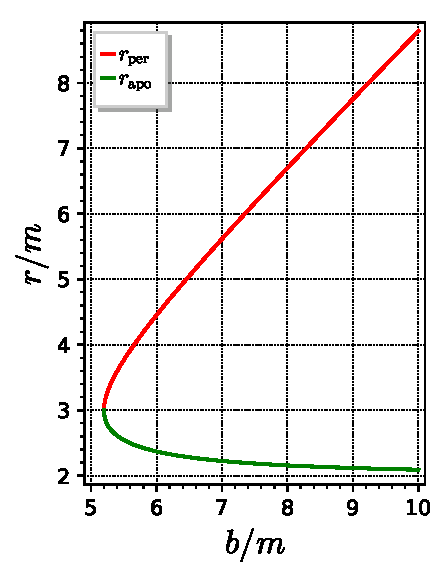
\includegraphics[width=0.4\textwidth]{ges_null_per_apo.pdf}}
\caption[]{\label{f:gis:null_per_apo} \footnotesize
Radial coordinate of the periastron, $r_{\rm p}$, and of the apoastron,
$r_{\rm a}$, along null geodesics with $b > b_{\rm c} \simeq 5.196\, m$.
Note that a given null geodesic has either a periastron or an apoastron, but not
both.}
\end{figure}

The variation of $r_{\rm p}$ and $r_{\rm a}$ with $b$ is plotted
in Fig.~\ref{f:gis:null_per_apo}. Note that $r_{\rm p} = r_{\rm a} = 3 m$
(the photon orbit) at the limit $b = b_{\rm c}$.
\begin{remark}
It is clear on Fig.~\ref{f:gis:null_per_apo} that, for the same value of $b$,
$r_{\rm a} \leq r_{\rm p}$, which may seem contradictory with the apoastron
corresponding to the largest distance from the center and the periastron to
the distance of closest approach.
However, one shall keep in mind that the apoastron and the periastron always refer to different null
geodesics: geodesics with an apoastron lie below the photon sphere ($r=3m$), while those
with a periastron are always outside it. A null geodesic can of course cross
the photon sphere (examples are geodesics 2 and 3 on Figs.~\ref{f:gis:eff_pot_null}
and \ref{f:gis:null_geod}), but then it has neither an apoastron nor a periastron
\end{remark}

%%%%%%%%%%%%%%%%%%%%%%%%%%%%%%%%%%%%%%%%%%%%%%%%%%%%%%%%%%%%%%%%%%%%%%%%%%%%%%%

\section{Trajectories of null geodesics in the equatorial plane} \label{s:gis:planar_trajectories}

In all this section, we assume $L\not = 0$, i.e. we consider non-radial
null geodesics, the radial case having been discussed in Sec.~\ref{s:gis:radial}.

Let us first recall the generic property of causal geodesics in Schwarzschild
spacetime established in Sec.~\ref{s:ges:eq_to_be_solved} : for $L\not=0$,
the azimuthal angle coordinate $\ph$ has no turning point: it is either always increasing
towards the future
($L>0$) or always decreasing towards the future ($L<0$).
\begin{remark}
We recover the above property from Eq.~(\ref{e:ges:dot_ph_null_b}):
$\D\ph/\D\tilde{\lambda} = \epsilon_L/r^2$, given that
$\epsilon_L = \operatorname{sgn} L$ and $\tilde{\lambda}$ increases towards
the future.
\end{remark}

\subsection{Differential equation and fundamental cubic polynomial}

The equation governing the $(r,\ph)$-part of a null geodesic, named
\emph{trajectory in the orbital plane} in Sec.~\ref{s:ges:trajectories},
is the generic differential equation (\ref{e:ges:DuDph_trajectories})
with $\mu$ (the particle's mass) set to zero and the ratio $E^2/L^2$ replaced
by $1/b^2$ [cf. Eq.~(\ref{e:ges:def_b})]:
\be \label{e:gis:du_dphi_null}
   \encadre{ \left( \frac{\D u}{\D \ph} \right)^2 = P_b(u)  }
\ee
where $u := m/r$ [Eq.~(\ref{e:ges:def_u})] and $P_b(u)$ stands for the cubic
polynomial
\be \label{e:ges:def_Pb_u}
      \encadre{  P_b(u) := 2 u^3 - u^2 + \frac{m^2}{b^2} } .
\ee
\begin{remark}
Of course, Eq.~(\ref{e:gis:du_dphi_null}) can be recovered by combining
Eqs.~(\ref{e:ges:dot_ph_null_b}), (\ref{e:ges:dot_r_square_null_b})
and (\ref{e:ges:eff_pot_null}).
\end{remark}



\begin{figure}
\centerline{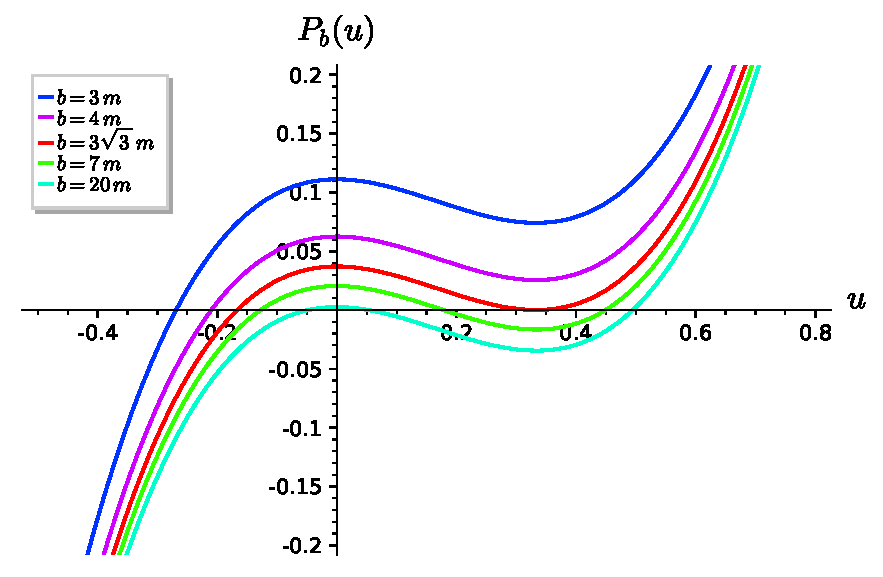
\includegraphics[width=0.7\textwidth]{ges_polynomial_b_u.pdf}}
\caption[]{\label{f:gis:polynomial_b_u} \footnotesize
Graph of the cubic polynomial $P_b(u) = 2 u^3 - u^2 + {m^2}/{b^2}$ [Eq.~(\ref{e:ges:def_Pb_u})].}
\end{figure}

By Eq.~(\ref{e:gis:du_dphi_null}), the zeros of the polynomial $P_b(u)$
correspond to points at which $\D u /\D\ph = 0$. They are thus stationary points
for $u$, and hence for $r$. This can only occur at the circular photon
orbit $r = \mathrm{const} = 3 m$ (then $b=b_{\rm c}$)
or at the periastron or apoastron discussed
in Sec.~\ref{s:ges:null_radial_behav} (then $b > b_{\rm c}$).
The graph of the polynomial $P_b(u)$ is shown in Fig.~\ref{f:gis:polynomial_b_u}
for selected values of $b$.
The zeros of $P_b(u)$ are governed by its
discriminant, which is
\be
    \Delta = 4 \frac{m^4}{b^4} \left( \frac{b^2}{m^2} - 27 \right) .
\ee
\begin{itemize}
\item If $\Delta<0$ $\iff$ $b <\sqrt{27} m = b_{\rm c}$,
$P_b(u)$ has one real negative zero and two complex zeros
(cf. blue and magenta curves in Fig.~\ref{f:gis:polynomial_b_u}),
so that it never vanishes
for physical values of $u$, which are real positive.
\item If $\Delta=0$ $\iff$ $b = b_{\rm c}$, $P_b(u)$
has a double zero: $u=1/3$ and a negative zero: $u=-1/6$ (cf. red curve
in Fig.~\ref{f:gis:polynomial_b_u}); only the first
one is physical and correspond to $r=3m$.
\item If $\Delta>0$ $\iff$ $b > b_{\rm c}$, $P_b(u)$ has three distinct
real zeros (cf. the green and cyan curves
in Fig.~\ref{f:gis:polynomial_b_u}); one of them, $u_{\rm n}$ say, is
negative, and hence unphysical, while the two others are positive, being nothing but
\be \label{e:ges:def_u_per_apo}
    u_{\rm p} = \frac{m}{r_{\rm p}} \qquad\mbox{and}\qquad
    u_{\rm a} = \frac{m}{r_{\rm a}} ,
\ee
where $r_{\rm p}$ and $r_{\rm a}$ are given by
Eqs.~(\ref{e:ges:sol_r_per})-(\ref{e:ges:sol_r_apo}).
\end{itemize}

\begin{figure}
\centerline{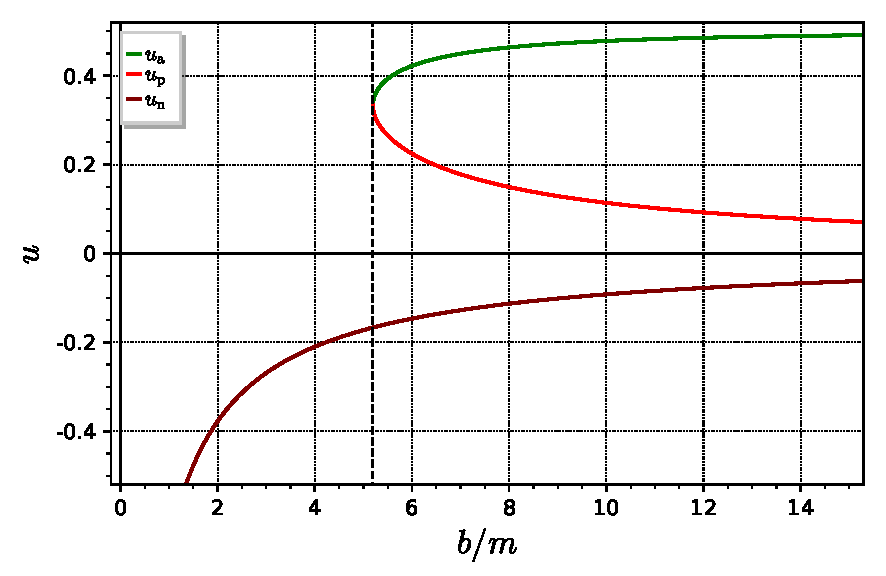
\includegraphics[width=0.7\textwidth]{gis_u_per_apo_neg.pdf}}
\caption[]{\label{f:gis:u_per_apo_neg} \footnotesize
Zeros $(u_{\rm n}, u_{\rm p}, u_{\rm a})$ of the cubic polynomial
$P_b(u) =  2 u^3 - u^2 + {m^2}/{b^2}$ as functions of $b$, for
$b\geq b_{\rm c} \simeq 5.196\, m$.}
\end{figure}

Since they will be required in what follows, let us
find explicit expressions for the real zeros of the polynomial $P_b$.
The equation $P_b(u) = 0$ can be brought to a depressed form (no square term)
by the change of variable $u = x + 1/6$. We get
\be \label{e:gis:zeros_Pb_eq_in_x}
    x^3 - \frac{1}{12} x + \frac{m^2}{2b^2} - \frac{1}{108} = 0 .
\ee
We shall discuss separately the cases $b>b_{\rm c}$ and $b<b_{\rm c}$.

\subsubsection{Zeros of $P_b$ for $b\geq b_{\rm c}$}

For $b>b_{\rm c}$, we can express the solutions of Eq.~(\ref{e:gis:zeros_Pb_eq_in_x})
via Viète's formulas \eqref{e:gis:Viete}
with $p = -1/12$ and $q = m^2/(2b^2) - 1/108$.
We then get the zeros of $P_b$ as
\[
    u_k = \frac{1}{3} \cos \left[ \frac{1}{3}
        \arccos \left( 1 - 2 \frac{b_{\rm c}^2}{b^2} \right) + \frac{2 k \pi}{3} \right]
        + \frac{1}{6},
        \qquad k \in \{0, 1, 2\} .
\]
Using the identity $\arccos(1 - 2 x^2) = 2\arcsin x$ and noticing
that $u_1 < 0$, which implies $u_1 = u_{\rm n}$, and $u_ 0 \geq u_2$, which
implies $u_0 = u_{\rm a}$ and $u_2 = u_{\rm p}$,
we arrive at
\begin{subequations}
\label{e:gis:zeros_Pbu}
\begin{align}
  &  \encadre{u_{\rm n} = \frac{1}{3}\cos\left[ \frac{2}{3} \arcsin\left(
   \frac{b_{\rm c}}{b}\right) + \frac{2\pi}{3}\right] + \frac{1}{6} } \qquad (b \geq b_{\rm c})\\[1ex]
 & \encadre{ u_{\rm p} = \frac{1}{3}\cos\left[ \frac{2}{3} \arcsin\left(
   \frac{b_{\rm c}}{b}\right) + \frac{4\pi}{3}\right] + \frac{1}{6} }
                            \label{e:gis:u_per_b} \qquad (b \geq b_{\rm c}) \\[1ex]
 & \encadre{ u_{\rm a} = \frac{1}{3}\cos\left[ \frac{2}{3} \arcsin\left(
   \frac{b_{\rm c}}{b}\right) \right] + \frac{1}{6} }  \qquad (b \geq b_{\rm c}) .
\end{align}
\end{subequations}
These zeros are plotted in term of $b$ on Fig.~\ref{f:gis:u_per_apo_neg}.
Note the ordering
\be \label{e:gis:order_u_zeros}
    -\frac{1}{6} \leq u_{\rm n} < 0 < u_{\rm p} \leq \frac{1}{3}
    \leq u_{\rm a} < \frac{1}{2} ,
\ee
with the inequalities $\leq$ being saturated for $b = b_{\rm c}$.

It is easy to express two of the zeros in terms of the third one. For instance,
let us pick $u_{\rm p}$. From $P_b(u_{\rm p}) = 0$, we have immediately
$b^2/m^2 = - 2 u_{\rm p}^3 + u_{\rm p}^2$. If we substitute this expression
for $b^2/m^2$ into $P_b(u)$, we get
\bea
    P_b(u) = 0 & \iff &  2 u^3 - u^2 - 2 u_{\rm p}^3 + u_{\rm p}^2 = 0  \nonumber \\
    & \iff & (u - u_{\rm p})\left[ 2 (u^2 + u_{\rm p} u + u_{\rm p}^2)
    - (u + u_{\rm p}) \right] = 0  \nonumber \\
    & \iff & (u - u_{\rm p})\left[ 2 u^2 + (2 u_{\rm p} - 1) u
      + u_{\rm p} (2 u_{\rm p} - 1) \right] = 0 . \nonumber
\eea
The two zeros different from $u_{\rm p}$ of this equation, namely
$u_{\rm n}$ and $u_{\rm a}$, must then obey
\[
    2 u^2 + (2 u_{\rm p} - 1) u
      + u_{\rm p} (2 u_{\rm p} - 1)  = 0 .
\]
Solving this quadratic equation leads to the sought expressions:
\begin{subequations}
\label{e:gis:una_up}
\begin{align}
u_{\rm n} & = \frac{1}{4} \left( 1 - 2 u_{\rm p}
    - \sqrt{(1 - 2 u_{\rm p} ) (1 + 6 u_{\rm p} )} \right) \\
u_{\rm a} & = \frac{1}{4} \left( 1 - 2 u_{\rm p}
    + \sqrt{(1 - 2 u_{\rm p} ) (1 + 6 u_{\rm p} )} \right) .
\end{align}
\end{subequations}


\subsubsection{Real zero of $P_b$ for $b<b_{\rm c}$}

As mentioned above, for $b<b_{\rm c}$, $P_b$ has only one real zero, $u_{\rm n}$,
which is negative. Its value is obtained by means of
\emph{Viète's substitution}\index{Viète's substitution},
which consists in setting $x = w + 1/(36 w)$ in Eq.~(\ref{e:gis:zeros_Pb_eq_in_x}),
thereby turning it into a quadratic equation for $w^3$. Solving the latter yields
\be
   \encadre{ u_{\rm n} = \frac{1}{6} \left[ 1
    - \left( \frac{b_{\rm c}}{b} - \sqrt{ \frac{b_{\rm c}^2}{b^2} - 1 } \right) ^{2/3}
    - \left( \frac{b_{\rm c}}{b} - \sqrt{ \frac{b_{\rm c}^2}{b^2} - 1 } \right) ^{- 2/3}
    \right] } \qquad (b < b_{\rm c}).
\ee



\subsection{Critical null geodesics} \label{s:gis:crit_geod}

For $b=b_{\rm c}$, the differential equation (\ref{e:gis:du_dphi_null})
can be integrated by means of elementary functions (Sec.~\ref{s:gis:crit_geod}),
while for $b \not= b_{\rm c}$,
it requires elliptic integrals of the first kind (Sec.~\ref{s:gis:gener_geod}).

Let us first consider the first case, i.e. assume $b = b_{\rm c} = 3\sqrt{3}\, m$.
Then $P_b(u) = (u - 1/3)^2 (2u + 1/3)$ and Eq.~(\ref{e:gis:du_dphi_null})
is equivalent to
\be \label{e:ges:dphi_du_null_bcrit}
    \frac{\D\ph}{\D u} = \pm \frac{1}{\left|u - \frac{1}{3}\right|
        \sqrt{2u+\frac{1}{3}}} .
\ee
This equation can be easily integrated by noticing that
\be \label{e:ges:primitive_crit_geod}
    \frac{1}{(1-x)\sqrt{x}} = \begin{cases}
       \displaystyle 2 \frac{\D}{\D x} \left( \mathrm{artanh}\, \sqrt{x} \right) \quad \mbox{for}\ x\in(0,1)\\[2ex]
       \displaystyle 2 \frac{\D}{\D x} \left( \mathrm{arcoth}\, \sqrt{x} \right) \quad \mbox{for}\ x\in(1,+\infty) .
    \end{cases}
\ee
We thus perform the change of variable $x=2u + 1/3$ and treat separately
two cases : $u<1/3 \iff x\in (1/3,1)$ and $u>1/3 \iff x\in (1,+\infty)$.
We call geodesics in the first case
\defin{external critical null geodesics}\index{external!critical null geodesic}\index{critical!null geodesic!external --},
since $u<1/3\iff r > 3 m$, and those in the second case
\defin{internal critical null geodesics}\index{internal!critical null geodesic}\index{critical!null geodesic!internal --},
since $u>1/3 \iff r < 3m$. The qualifiers \emph{external} and \emph{internal} thus refer
to the photon sphere $r=3 m$ discussed in Sec.~\ref{s:ges:null_eff_pot}.

\begin{figure}
\centerline{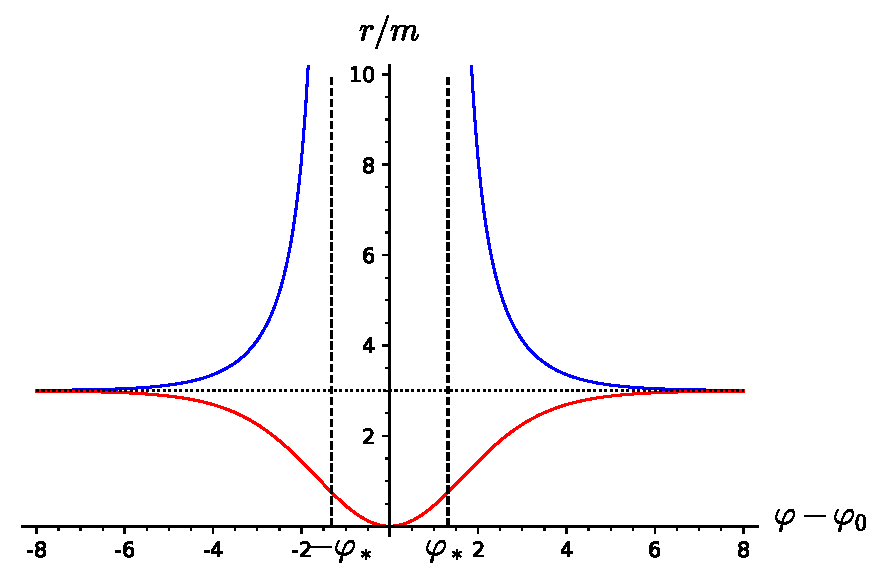
\includegraphics[width=0.7\textwidth]{ges_null_r_phi_bcrit.pdf}}
\caption[]{\label{f:gis:null_r_phi_bcrit} \footnotesize
$r$ as a function of $\ph$ along a null geodesic with an impact parameter
equal to the critical one:
$b = b_{\rm c} = 3\sqrt{3} \, m$; the blue curve is for a critical
null geodesic with $r>3m$
[Eq.~(\ref{e:ges:null_r_phi_tanh})], while the red one
regards $r<3m$ [Eq.~(\ref{e:ges:null_r_phi_coth})].}
\end{figure}

\subsubsection{External critical null geodesics} \label{s:gis:extern_crit_geod}

For $u<1/3$, $x\in(1/3, 1)$, so that the first line of Eq.\eqref{e:ges:primitive_crit_geod}
is relevant and Eq.~\eqref{e:ges:dphi_du_null_bcrit} is integrated to
\be \label{e:ges:ph_u_crit_null_geod}
    \ph = \pm 2 \,\mathrm{artanh}\, \sqrt{2u + \frac{1}{3}} + \ph_0 ,
\ee
where $\ph_0$ is some integration constant. This relation is easily inverted
to
\be \label{e:ges:u_ph_crit_null_geod}
    u = \frac{1}{2}  \tanh^2 \left(\frac{\ph - \ph_0}{2} \right) - \frac{1}{6} .
\ee
Moving back to $r = m/u$, we obtain the equation of the external critical
null geodesic in polar form:
\be \label{e:ges:null_r_phi_tanh}
   \encadre{ r = \frac{2m}{\tanh^2 \left(\frac{\ph - \ph_0}{2} \right) - \frac{1}{3}} }.
\ee
The constant $\ph_0$ can be related to the asymptotic value $\ph_\infty$ of $\ph$
when $r\to +\infty$ by setting $u=0$ in Eq.~(\ref{e:ges:u_ph_crit_null_geod});
we get, using the identity $\mathrm{artanh}\,  x = 1/2\ln[(1+x)/(1-x)]$,
\be \label{e:ges:null_ph_0_ph_inf}
    \ph_0 = \ph_\infty \pm \ph_*,\quad\mbox{with}\quad
    \ph_* := \ln\left(\frac{\sqrt{3} + 1}{\sqrt{3} - 1}\right)
    \simeq 1.316958.
\ee

The function $r(\ph)$, as given by Eq.~(\ref{e:ges:null_r_phi_tanh}), is
depicted on Fig.~\ref{f:gis:null_r_phi_bcrit} (blue curve).
The region $\ph_0-\ph_* < \ph < \ph_0 + \ph_*$ is excluded, since
Eq.~(\ref{e:ges:null_r_phi_tanh}) would yield $r<0$. For $\ph > \ph_0 + \ph_*$,
$r(\ph)$ is a decaying
function, which corresponds to the
plus sign in Eq.~(\ref{e:ges:ph_u_crit_null_geod}) and to the minus sign in
Eq.~(\ref{e:ges:null_ph_0_ph_inf}): $\ph_0 = \ph_\infty - \ph_*$.
Figure~\ref{f:gis:null_b_crit_from_inf_L_pos} shows such a null geodesic with
$\ph_\infty=0$, which implies $\ph_0 = - \ph_*$ and $\ph>0$.
When $\ph\to +\infty$, the geodesic rolls up indefinitely onto the photon
orbit discussed in Sec.~\ref{s:ges:null_eff_pot}; this
behaviour corresponds to the horizontal asymptote at $r=3m$ in
the right part of Fig.~\ref{f:gis:null_r_phi_bcrit}.
Note that the geodesic approaches very fast the photon orbit, only a single
path round to it being graphically visible in Fig.~\ref{f:gis:null_b_crit_from_inf_L_pos}.
This is because the asymptotic expansion of relation~\eqref{e:ges:null_r_phi_tanh} is
$r\sim 3m(1+ 6\mathrm{e}^{-\ph})$ when $\ph\to+\infty$.

It is worth stressing that Fig.~\ref{f:gis:null_b_crit_from_inf_L_pos} describes both (i) the trace
in the $(x,y)$-plane of a
geodesic with $L>0$ (so that $\ph$ increases towards the future, cf. Eq.~(\ref{e:ges:dot_ph_null})) arising from $r\to + \infty$
and spiralling inwards to the photon orbit
and (ii) the trace of a geodesic with $L<0$ (so that $\ph$ decays towards the future)
arising from $r=r_{\rm em} > 3 m$, $\ph=\ph_{\rm em}>0$,
spiralling outwards and escaping to $r\to +\infty$ as $\ph\to 0$. Had we restored the
$t$ dimension perpendicular to the $(x,y)$-plane in a 3d plot, these two geodesics would have
clearly appeared distinct.

\begin{figure}
\centerline{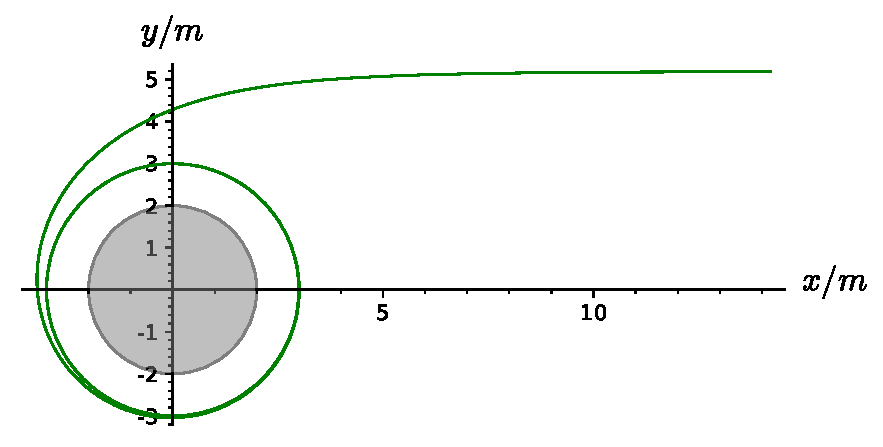
\includegraphics[width=0.7\textwidth]{ges_null_b_crit_from_inf_L_pos.pdf}}
\caption[]{\label{f:gis:null_b_crit_from_inf_L_pos} \footnotesize
Trace in the equatorial plane spanned by the coordinates $x:=r\cos\ph$, $y:=r\sin\ph$
of an external critical null geodesic ($b = 3\sqrt{3} \, m \simeq 5.196 m$ and
$r>3m$) with $\ph_\infty=0$.
It obeys Eq.~(\ref{e:ges:null_r_phi_tanh}) with $\ph_0 = -\ph_*$ and $\ph\in(0,+\infty)$
(right branch of the blue curve in Fig.~\ref{f:gis:null_r_phi_bcrit}).}
\end{figure}

\begin{figure}
\centerline{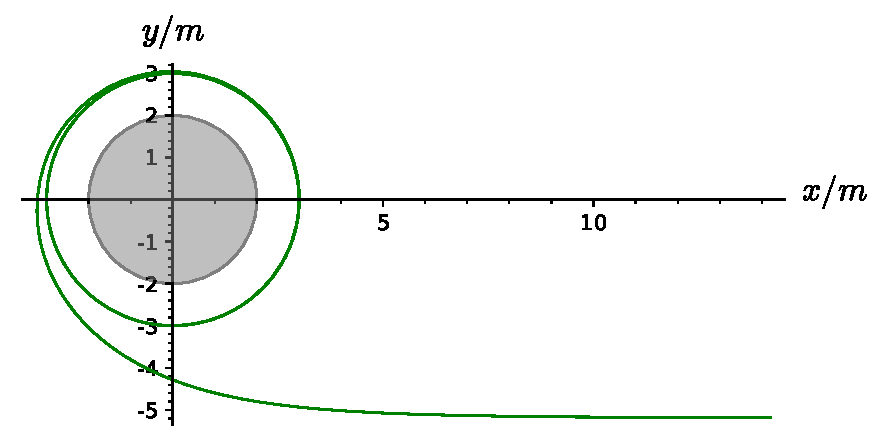
\includegraphics[width=0.7\textwidth]{ges_null_b_crit_from_inf_L_neg.pdf}}
\caption[]{\label{f:gis:null_b_crit_from_inf_L_neg} \footnotesize
Same as Fig.~\ref{f:gis:null_b_crit_from_inf_L_pos}, but for $\ph_0 = \ph_*$
and $\ph\in(-\infty,0)$ (left branch of the blue curve in Fig.~\ref{f:gis:null_r_phi_bcrit}).}
\end{figure}

On the contrary, for $\ph < \ph_0 - \ph_*$,
$r(\ph)$ is an increasing
function, as it is clear on the left part of the blue curve in Fig.~\ref{f:gis:null_r_phi_bcrit}.
This corresponds to the
minus sign in Eq.~(\ref{e:ges:ph_u_crit_null_geod}) and to the plus sign in
Eq.~(\ref{e:ges:null_ph_0_ph_inf}): $\ph_0 = \ph_\infty + \ph_*$.
A null geodesic of this type is depicted in Fig.~\ref{f:gis:null_b_crit_from_inf_L_neg}.
It has $\ph_\infty = 0$, so that $\ph_0 = \ph_*$ and $\ph < 0$.
As for Fig.~\ref{f:gis:null_b_crit_from_inf_L_pos}, the curve depicted in
Fig.~\ref{f:gis:null_b_crit_from_inf_L_neg} can be interpreted as the trace
in the $(x,y)$-plane of two distinct
geodesics: one with $L<0$ arising from $r\to + \infty$
and spiralling inwards to the photon orbit when $\ph\to -\infty$
and another one with $L>0$
arising from $r=r_{\rm em} > 3 m$, $\ph=\ph_{\rm em}<0$,
spiralling outwards and escaping to $r\to +\infty$ as $\ph\to 0$.

\begin{figure}
\centerline{
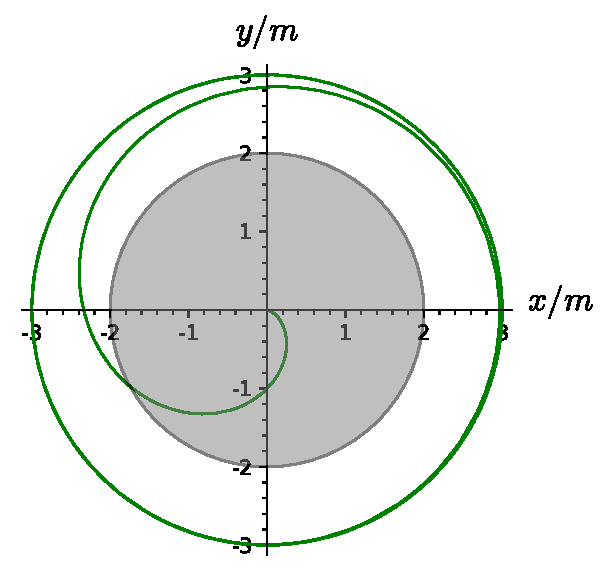
\includegraphics[width=0.35\textwidth]{ges_null_b_crit_intern_1.pdf}\qquad
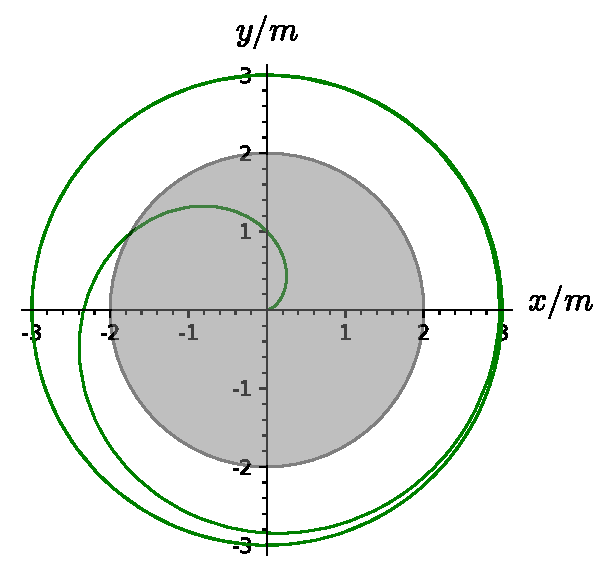
\includegraphics[width=0.35\textwidth]{ges_null_b_crit_intern_2.pdf}
}
\caption[]{\label{f:gis:null_b_crit_intern} \footnotesize
Trace in the equatorial plane of two internal critical null geodesics ($b = 3\sqrt{3} \, m \simeq 5.196 m$ and
$r<3m$). They both obey Eq.~\eqref{e:ges:null_r_phi_coth} with $\ph_0 = 0$.
The left panel corresponds to $\ph\in (-\infty, 0)$ (left part of the red curve
in Fig.~\ref{f:gis:null_r_phi_bcrit}), while the right one is
for $\ph\in (0, +\infty)$ (right part of the red curve
in Fig.~\ref{f:gis:null_r_phi_bcrit}).}
\end{figure}


\subsubsection{Internal critical null geodesics}

Let us now consider the ``internal'' case: $r< 3m \iff u>1/3$.
This implies $x\in (1,+\infty)$ in Eq.~\eqref{e:ges:primitive_crit_geod},
so that Eq.~\eqref{e:ges:dphi_du_null_bcrit} is integrated to
\be \label{e:ges:null_r_phi_coth}
    \encadre{ r = \frac{2m}{\coth^2 \left(\frac{\ph - \ph_0}{2} \right) - \frac{1}{3}} }.
\ee
Again, $\ph_0$ is an integration constant. But this time, it cannot be determined by the
value of $\ph$ when $r\to +\infty$ since we are in the case $r<3m$.
The function $r(\ph)$ given by Eq.~\eqref{e:ges:null_r_phi_coth} is plotted as the red
curve in Fig.~\ref{f:gis:null_r_phi_bcrit}. Contrary to external critical null geodesics, there
is no exclusion interval for $\ph$. However, $\ph$ cannot range from $-\infty$
to $+\infty$ along a given geodesic. Indeed, for $\ph=\ph_0$, one gets
$r=0$, which corresponds to the curvature singularity of the Schwarzschild black hole.
This is necessarily a termination point for any geodesic. The maximum
range of $\ph$ along an internal critical null geodesic is therefore
either $(-\infty,\ph_0)$ or $(\ph_0,+\infty)$.

An internal critical null geodesic with $\ph_0=0$ and $\ph\in(-\infty,0)$
is depicted in the left panel of Fig.~\ref{f:gis:null_b_crit_intern}.
For $\ph\to -\infty$, it rolls up indefinitely onto the photon
orbit ($r=3m$) from below. Again the approach to the photon orbit is exponentially
fast, the asymptotic expansion of relation \eqref{e:ges:null_r_phi_coth} being
$r\sim 3m (1 - 6 \mathrm{e}^\ph)$ when $\ph\to -\infty$.
The curve plotted in Fig.~\ref{f:gis:null_b_crit_intern} actually represents the trace in the equatorial plane of two
distinct geodesics: (i) a geodesic with $L>0$ arising
from $r=r_{\rm em} < 3 m$, $\ph=\ph_{\rm em}<0$ and inspiralling to the
central singularity as $\ph\to 0$ and (ii) a geodesic with $L<0$ arising from
$r = r_{\rm em} \in (2m,  3 m)$, $\ph=\ph_{\rm em}<0$ and spiralling outward
to the photon orbit as $\ph\to -\infty$. Note that for (ii), the
emission point must fulfil $r_{\rm em} > 2m$, i.e. must lie outside the black
hole region. Indeed, as shown in Sec.~\ref{s:ges:eq_to_be_solved}, along
any geodesic, $r$ must decrease towards the future in the black hole region.
Hence no null geodesic can be spiralling outwards there.

The right panel of Fig.~\ref{f:gis:null_b_crit_intern} corresponds to an
internal critical null geodesic with $\ph_0=0$ and $\ph\in(0, \infty)$.
For $\ph\to +\infty$, it rolls up indefinitely onto the photon
orbit ($r=3m$) from below. Again, the plotted curve describes two cases:
(i) a geodesic with $L<0$ arising
from $r=r_{\rm em} < 3 m$, $\ph=\ph_{\rm em}>0$ and inspiralling to the
central singularity as $\ph\to 0$ and (ii) a geodesic with $L>0$ arising from
$r = r_{\rm em} \in (2m,  3 m)$, $\ph=\ph_{\rm em}>0$ and spiralling outward
to the photon orbit as $\ph\to +\infty$.


\subsection{Generic null geodesics} \label{s:gis:gener_geod}

As stated above, for $b \not= b_{\rm c}$, the differential equation~\eqref{e:gis:du_dphi_null} cannot be integrated
in terms of elementary functions. It is integrable though in terms of standard
functions of mathematical physics, namely elliptic integrals of the first kind.
As a first step, we rewrite Eq.~(\ref{e:gis:du_dphi_null}) as
\be \label{e:ges:dphi_du_null}
   \frac{\D\ph}{\D u} = \pm \frac{1}{\sqrt{2 u^3 - u^2 + (m/b)^2}}  ,
\ee
where the $\pm$ sign is
\begin{itemize}
\item $+$ if (i) $L>0$ and $r$ is decreasing (towards the future) along the geodesic
$\Li$ at the considered point or (ii) $L<0$ and $r$ is increasing along $\Li$;
\item $-$ if (i) $L>0$ and $r$ is increasing along $\Li$ or (ii)
$L<0$ and $r$ is decreasing along $\Li$.
\end{itemize}


We shall consider only geodesics with $b>b_{\rm c}$ and outside
the photon sphere, because they are the most
relevant ones for the images to be discussed in Sec.~\ref{s:gis:images}.
Each of these geodesics has a periastron and obeys $u\to 0$
($r\to +\infty$) for both $\tlamb\to -\infty$ and
$\tlamb\to +\infty$. We naturally denote by $\tlamb_{\rm p}$ the value of the
affine parameter $\tlamb$ at the periastron.

Let us first consider a null geodesic $\Li$ with $L>0$. On the part prior to
the periastron, i.e. for $\tlamb \leq \tlamb_{\rm p}$, one has
$\D\ph > 0$ and $\D u \geq 0$, so that the $+$ sign must be selected in
Eq.~(\ref{e:ges:dphi_du_null}) and its solution can be written as
\[
    \ph = \ph_{-\infty} + \int_0^u \frac{\D\bar{u}}{\sqrt{P_b(\bar{u})}} ,
\]
where $\ph_{-\infty} := \lim_{\tlamb\to-\infty} \ph$ since, being outside
the photon sphere, the geodesic arises from infinity where $u := m/r = 0$.
We shall rewrite the above expression as
\be
    \ph = \ph_{-\infty} + \Phi_b(0) - \Phi_b(u) \qquad (L>0,\ \tlamb \leq \tlamb_{\rm p}),
\ee
where we have introduced the function
\be
   \encadre{  \Phi_b(u) := \int_u^{u_{\rm p}} \frac{\D\bar{u}}{\sqrt{P_b(\bar{u})}}
      = \int_u^{u_{\rm p}} \frac{\D\bar{u}}{\sqrt{2 \bar{u}^3 - \bar{u}^2 + (m/b)^2}} } .
\ee
Since $u_{\rm p}$ is the function of $b$ given by Eq.~\eqref{e:gis:u_per_b},
the above relation defines uniquely a function of $u$ and $b$, which we consider
as a function of $u$ parametrized by $b$.

In the part of $\Li$ past to the periastron, one has $\D\ph > 0$ and $\D u < 0$,
so that the $-$ sign must be selected in Eq.~(\ref{e:ges:dphi_du_null}); accordingly,
the solution for $\tlamb > \tlamb_{\rm p}$ can be written as
\[
    \ph = \ph_{-\infty} +  \int_0^{u_{\rm p}} \frac{\D\bar{u}}{\sqrt{P_b(\bar{u})}}
        - \int_{u_{\rm p}}^u \frac{\D\bar{u}}{\sqrt{P_b(\bar{u})}}
        = \ph_{-\infty} + \int_0^{u_{\rm p}} \frac{\D\bar{u}}{\sqrt{P_b(\bar{u})}}
         + \int_u^{u_{\rm p}} \frac{\D\bar{u}}{\sqrt{P_b(\bar{u})}}.
\]
Hence
\be
    \ph = \ph_{-\infty} + \Phi_b(0) + \Phi_b(u) \qquad (L>0,\ \tlamb > \tlamb_{\rm p}) .
\ee
For a null geodesic with $L < 0$, a similar reasoning with $\D\ph > 0$
changed to $\D\ph < 0$ leads to
\be
    \ph = \ph_{-\infty} + \Phi_b(u) - \Phi_b(0) \qquad (L<0,\ \tlamb \leq \tlamb_{\rm p}),
\ee
\be
    \ph = \ph_{-\infty} - \Phi_b(u) - \Phi_b(0)  \qquad (L<0,\ \tlamb > \tlamb_{\rm p}) .
\ee
We may combine the above results into
\be \label{e:gis:ph_Phi_b_u}
   \encadre{ \ph =  \ph_{-\infty} + \begin{cases}
       \displaystyle \epsilon_L(\Phi_b(0) - \Phi_b(u)) \quad \mbox{for}\
            \tlamb \leq \tlamb_{\rm p}\\[2ex]
       \displaystyle \epsilon_L(\Phi_b(0) + \Phi_b(u)) \quad \mbox{for}\
            \tlamb > \tlamb_{\rm p}
    \end{cases} }
\ee
It thus appears that
$\ph$ is entirely determined by the function $\Phi_b(u)$. To evaluate
the latter, we rewrite it in terms of the three zeros
$(u_{\rm n}, u_{\rm p}, u_{\rm a})$ of $P_b(u)$:
\be \label{e:gis:Phi_b_int_Pb_zeros}
  \Phi_b(u) = \int_u^{u_{\rm p}} \frac{\D\bar{u}}{
  \sqrt{2(\bar{u} - u_{\rm n})(u_{\rm p} - \bar{u})(u_{\rm a} - \bar{u})}} .
\ee
We then perform the change of variable\footnote{It should be clear that the
variable $t$ introduced here has nothing to do with the Schwarzschild-Droste
coordinate $t$.}
\be
    t := \frac{1}{k} \sqrt{\frac{u_{\rm p} - \bar{u}}{u_{\rm a} - \bar{u}}}
    \quad\iff\quad
    \bar{u} = \frac{u_{\rm p} - u_{\rm a} k^2 t^2}{1 - k^2 t^2} ,
\ee
where $k$ is the following constant:
\be \label{e:gis:def_k_modulus}
   \encadre{ k := \sqrt{\frac{u_{\rm p} - u_{\rm n}}{u_{\rm a} - u_{\rm n}}}
    = \frac{\sqrt{2}}{
       \sqrt{\sqrt{3}\cot\left(\frac{2}{3}\arcsin\left(\frac{b_{\rm c}}{b}\right)\right) + 1}}},
\ee
where the second equality follows from the expressions \eqref{e:gis:zeros_Pbu}
of $u_{\rm n}$, $u_{\rm p}$ and
$u_{\rm a}$ in terms of $b$.
Noticing that
\[
    \D\bar{u} = - \frac{2(u_{\rm a} - u_{\rm p}) k^2 t}{(1 - k^2 t^2)^2} \, \D t,
    \qquad
    \bar{u} - u_{\rm n} = \frac{(u_{\rm p} - u_{\rm n})(1 -t^2)}{1 - k^2 t^2} ,
\]
\[
   u_{\rm p} - \bar{u} =
    \frac{(u_{\rm p} - u_{\rm n})(u_{\rm a} - u_{\rm p}) t^2}{
    (u_{\rm a} - u_{\rm n})(1 - k^2 t^2)}
    \quad\mbox{and}\quad
    u_{\rm a} - \bar{u} = \frac{u_{\rm a} - u_{\rm p}}{1 - k^2 t^2} ,
\]
we get
\be
     \Phi_b(u) = \frac{\sqrt{2}}{\sqrt{u_{\rm a} - u_{\rm n}}}
     \int_0^{\frac{1}{k} \sqrt{\frac{u_{\rm p} - u}{u_{\rm a} - u}}}
     \frac{\D t}{\sqrt{(1 - t^2)(1 - k^2 t^2)}} .
\ee
The term $\D t/\sqrt{1 - t^2}$ suggests to perform the change of
variable $t = \sin\vartheta$. We then arrive at
\be \label{e:gis:Phib_elliptic_int}
    \encadre{ \Phi_b(u) = \frac{\sqrt{2}}{\sqrt{u_{\rm a} - u_{\rm n}}}
    \, F\left(
    \arcsin\left( \frac{1}{k} \sqrt{\frac{u_{\rm p} - u}{u_{\rm a} - u}}\right),\;
        k\right) } ,
\ee
where $F(\phi, k)$ is the
\defin{incomplete elliptic integral of the first kind}\index{incomplete!elliptic integral}\index{elliptic integral!incomplete --}:
\be \label{e:gis:def_incompl_elliptic_int}
    F(\phi, k) := \int_0^\phi \frac{\D\vartheta}{\sqrt{1 - k^2 \sin^2\vartheta}} .
\ee
The notation $F(\phi, k)$ is the most commonly used
in the literature \cite{ByrdF71,GradsRGTJ115}, but one may encounter as well
$F(\phi|m)$ for $F(\phi, k)$ with $m=k^2$ \cite{AbramS72}.
$k$ is called the \defin{modulus}\index{modulus!of an elliptic integral} of
the elliptic integral. From its expression \eqref{e:gis:def_k_modulus}, we
see that $k$ is a function of $b$. It is plotted in Fig.~\ref{f:gis:elliptic_mod}.
Given the ordering \eqref{e:gis:order_u_zeros}, we deduce from
\eqref{e:gis:def_k_modulus} that
\be
    0 < k \leq 1,
\ee
with $k=1 \iff u_{\rm p} = u_{\rm a} \iff b = b_{\rm c}$.
\begin{figure}
\centerline{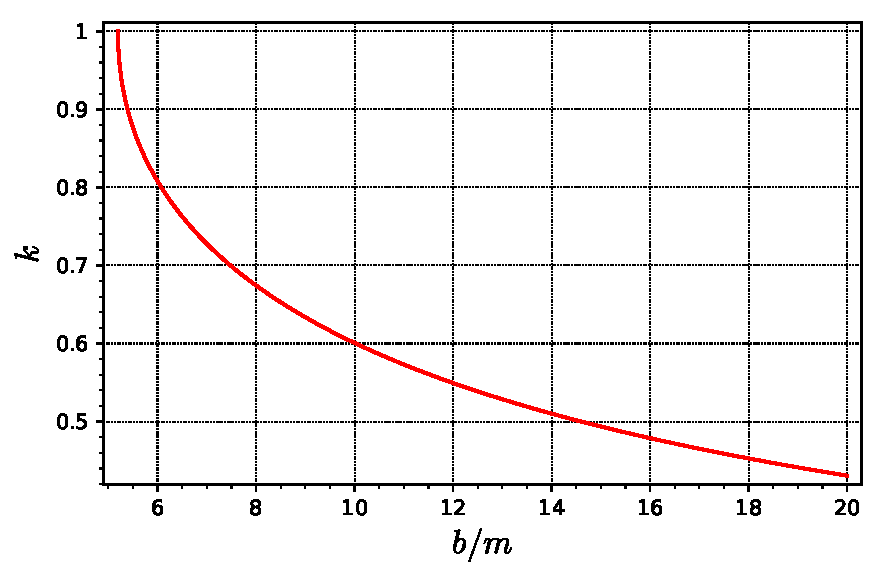
\includegraphics[width=0.7\textwidth]{gis_elliptic_mod.pdf}}
\caption[]{\label{f:gis:elliptic_mod} \footnotesize
Modulus $k$ of the incomplete elliptic integral $F$ that is involved
in expression (\ref{e:gis:Phib_elliptic_int}) for $\Phi_b(u)$.}
\end{figure}



\begin{remark}
The trajectory of a null geodesic in the plane $\th=\pi/2$ as given by
Eqs.~(\ref{e:gis:ph_Phi_b_u}) and (\ref{e:gis:Phib_elliptic_int})
is of the form $\ph = \ph(r)$
on each of the two arcs with respect to the periastron. One can invert
this relation to express the trajectory in the polar form $r = r(\ph)$. This
is performed thanks to the inverse of the incomplete elliptic integral $F(\phi,k)$,
which is the \defin{Jacobi elliptic sine}\index{Jacobi!elliptic sine}\index{elliptic!sine}
$\operatorname{sn}(x,k)$, defined by $\sin\phi = \operatorname{sn}(F(\phi,k), k)$. We deduce then
from Eq.~(\ref{e:gis:Phib_elliptic_int}) that
\be
    \frac{u_{\rm p} - u}{u_{\rm a} - u} = k^2 \operatorname{sn}\left(
    \frac{\sqrt{u_{\rm a} - u_{\rm n}}}{\sqrt{2}} \Phi_b(u),\; k \right) .
\ee
We refer the reader to Refs.~\cite{CadezK05,Munoz14} for more details.
\end{remark}

\subsection{Deflection angle and winding number} \label{s:gis:deflect_winding}

The total change of $\ph$ along the geodesic history is
\be
    \Delta \ph = \ph_\infty - \ph_{-\infty} ,
\ee
with $\ph_\infty := \lim_{\tlamb\to +\infty} \ph$.
Given that $\lim_{\tlamb\to +\infty} u = 0$ (since $b>b_{\rm c}$, the geodesic
is escaping to infinity), Eq.~\eqref{e:gis:ph_Phi_b_u} leads to
\[
    \ph_\infty = \ph_{-\infty} + \epsilon_L (\Phi_b(0) + \Phi_b(0)) .
\]
Hence
\be \label{e:gis:Dph_Phi_b_0}
    \Delta\ph = 2 \epsilon_L \Phi_b(0) .
\ee
Given the expression  (\ref{e:gis:Phib_elliptic_int}) of $\Phi_b$, we
get
\be \label{e:gis:Dph_F_psi_k}
    \encadre{  \Delta\ph = \epsilon_L \frac{2 \sqrt{2}}{\sqrt{u_{\rm a} - u_{\rm n}}}
    \, F(\psi, k) } ,
\ee
where
\be \label{e:gis:def_psi}
   \encadre{ \psi := \arcsin\left( \frac{1}{k} \sqrt{\frac{u_{\rm p}}{u_{\rm a}}} \right) } .
\ee

Note that one can have $|\Delta\ph| > 2\pi$; in such a case, the null geodesic
is winding around the black hole before leaving to infinity. We therefore introduce
the \defin{winding number}\index{winding!number!of null geodesic} $n\in\mathbb{Z}$ by
\be \label{e:gis:def_Dph_bar}
    \Delta\ph =: \overline{\Delta\ph} + 2\pi n \quad
    \mbox{with} \quad
    \begin{cases}
    \overline{\Delta\ph} \in [0, 2\pi) &\  \mbox{if}\ L > 0 \\
    \overline{\Delta\ph} \in (-2\pi, 0] &\  \mbox{if}\ L < 0 .
    \end{cases}
\ee
Note that $n\geq 0$ for $L > 0$ and $n\leq 0$ for $L<0$.
We then define the \defin{deflection angle}\index{deflection!angle}
$\Theta$ by
\be \label{e:gis:def_deflection_angle}
    \Theta := \overline{\Delta\ph} - \epsilon_L \pi .
\ee
Let us recall that $\epsilon_L = \pm 1$ is the sign of the
conserved angular momentum $L$ [cf. Eq.~(\ref{e:gis:def_epsilon_L})].
The $-\epsilon_L \pi$ term in the above equation is chosen so
that $\Theta = 0$ in flat spacetime (no deflection of light).
By construction, the range of $\Theta$ is
\be
    -\pi \leq \Theta \leq \pi .
\ee


\begin{figure}
\begin{tabular}{cc}
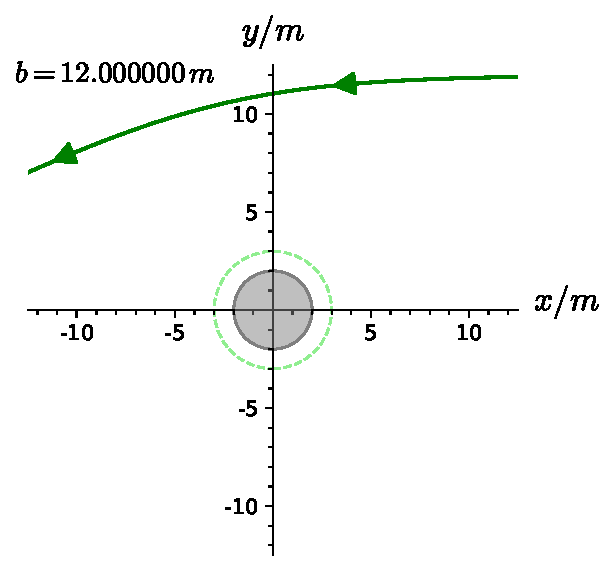
\includegraphics[width=0.48\textwidth]{ges_null_b_12_000000.pdf} &
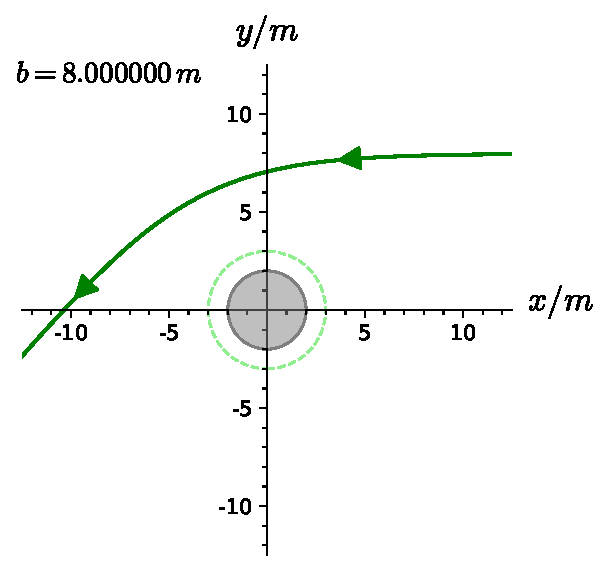
\includegraphics[width=0.48\textwidth]{ges_null_b_8_000000.pdf} \\
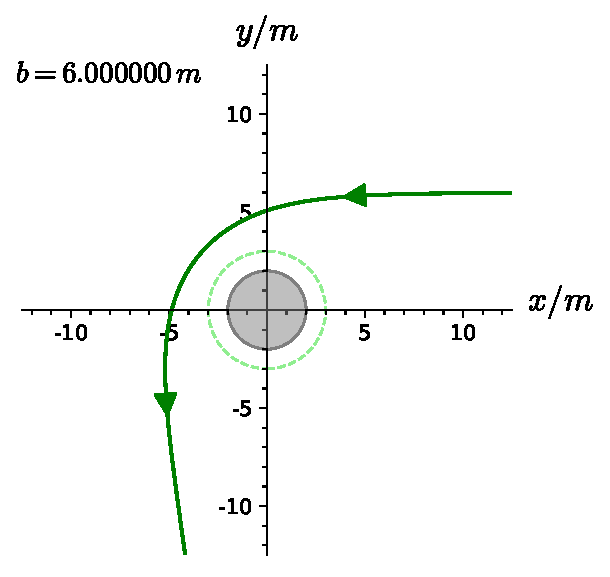
\includegraphics[width=0.48\textwidth]{ges_null_b_6_000000.pdf} &
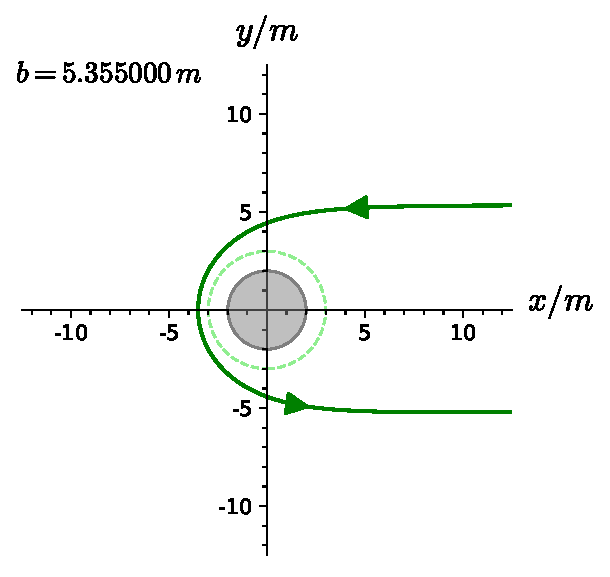
\includegraphics[width=0.48\textwidth]{ges_null_b_5_355000.pdf}
\end{tabular}
\caption[]{\label{f:gis:null_b1} \footnotesize
Null geodesics in the equatorial plane of Schwarzschild spacetime,
plotted in terms of the coordinates $(x,y) := (r\cos\ph, r\sin\ph)$,
arising from $x\gg m$ with trajectories all initially parallel to the $x$-axis,
but differing by the value of the impact parameter $b$.
The grey disk marks the black hole
region $r<2m$, while the dashed green circle indicates the photon orbit
at $r=3m$.}
\end{figure}

\begin{figure}
\begin{tabular}{cc}
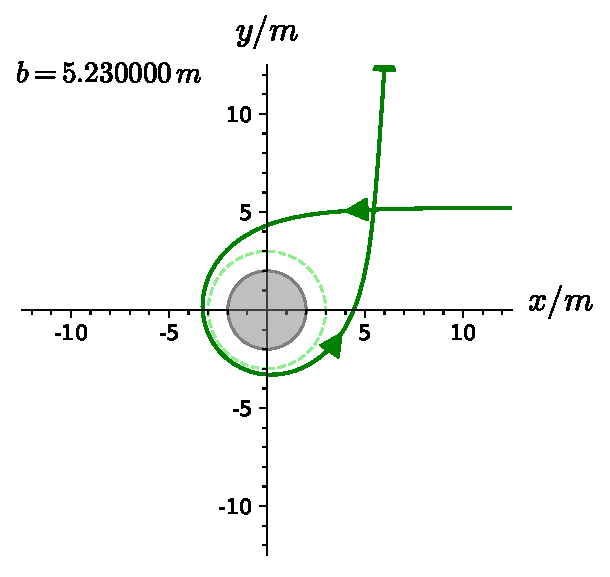
\includegraphics[width=0.48\textwidth]{ges_null_b_5_230000.pdf} &
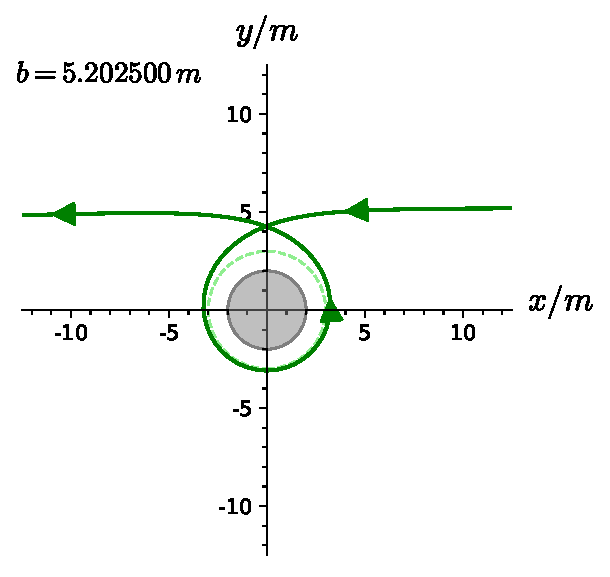
\includegraphics[width=0.48\textwidth]{ges_null_b_5_202500.pdf} \\
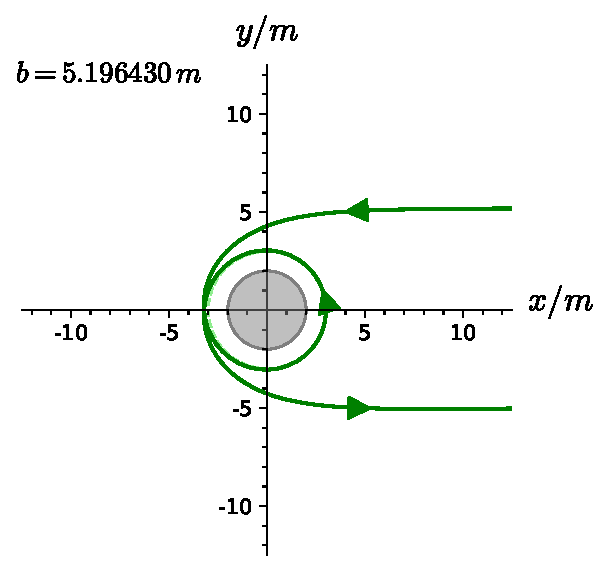
\includegraphics[width=0.48\textwidth]{ges_null_b_5_196430.pdf} &
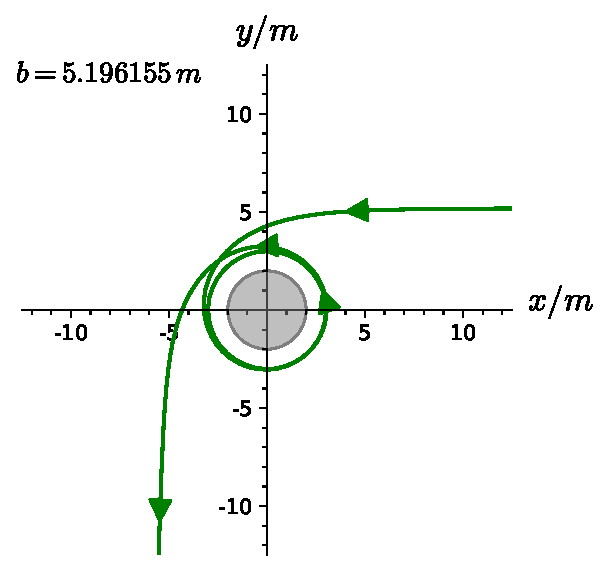
\includegraphics[width=0.48\textwidth]{ges_null_b_5_196155.pdf}
\end{tabular}
\caption[]{\label{f:gis:null_b2} \footnotesize
Same as Fig.~\ref{f:gis:null_b1} but for values of $b$ closer to
$b_{\rm c} \simeq 5.196152\, m$.}
\end{figure}

The above concepts are illustrated in Figs.~\ref{f:gis:null_b1}-\ref{f:gis:null_b2},
which show the trajectories
of null geodesics arising from infinity along the
direction $\ph=0$ (i.e. having $\ph_{-\infty=0}$, for various values of the
impact parameter $b$ decaying from $b=12 m$ to $b_{\rm c}$.
They have been computed by means of the geodesic integrator
of \textsf{SageMath} (cf. Appendix~\ref{s:sam}), instead of making use
of the elliptic integral (\ref{e:gis:Phib_elliptic_int}).
All these geodesics have $L>0$ and hence $\epsilon_L = +1$.
For $b=12 m$ (upper left panel of Fig.~\ref{f:gis:null_b1}),
the geodesic suffers only some moderate bending; this is nothing but the standard
\defin{deflection of light}\index{deflection of light} by massive bodies in
general relativity. More precisely, we have in this case $\Theta\simeq \pi/6$ and $n=0$.
For $b=8 m$ and $6 m$, the bending is more pronounced,
exceeding $\Theta = \pi/2$ for $b=6 m$, still with $n=0$. For $b=5.355\, m$ (lower right panel of Fig.~\ref{f:gis:null_b1}), the deflection angle is $\Theta\simeq\pi$, i.e. the photon goes back in the direction
from which it was coming.

When the impact parameter becomes even closer to the critical value
$b_{\rm c}\simeq 5.196152\, m$ [Eq.~(\ref{e:ges:b_crit})],
the null geodesic starts to wind around the black hole before escaping
to infinity (Fig.~\ref{f:gis:null_b2}).
For $b=5.230\, m$ (upper left panel of Fig.~\ref{f:gis:null_b2}), one has
$n=1$ and $\Theta\simeq -\pi/2$.
For $b=5.2025\, m$ (upper right panel of Fig.~\ref{f:gis:null_b2}), one has
$n=1$ and $\Theta=0$. For $b=5.19643\, m$ (lower left panel
of Fig.~\ref{f:gis:null_b2}), one has
$n=1$ and $\Theta\simeq \pi$ and for $b=5.196155\, m$ (lower right panel of Fig.~\ref{f:gis:null_b2}), one has $n=2$ and
$\Theta\simeq \pi/2$.
Note that the winding is taking place
almost at the photon circular orbit ($r=3m$). That after a few turns the null geodesic
departs to infinity corroborates the fact that the photon orbit is unstable
(cf. Sec.~\ref{s:ges:null_eff_pot}).

We can understand the winding phenomenon
around the photon circular orbit for $b$ close to $b_{\rm c}$
without investigating the properties of elliptic integrals.
Indeed, by combining Eqs.~(\ref{e:gis:Dph_Phi_b_0}) and (\ref{e:gis:Phi_b_int_Pb_zeros}),
we get
\be \label{e:ges:Dph_u_per_apo}
    \Delta\ph = \epsilon_L \sqrt{2} \int_0^{u_{\rm p}}
    \frac{\D u}{\sqrt{(u_{\rm p} - u )(u_{\rm a} - u)(u - u_{\rm n})}} .
\ee
Given the ordering (\ref{e:gis:order_u_zeros}), each of the
three terms under the square root is positive on the integration range
$(0,u_{\rm p})$. For $b\not=b_{\rm c}$, $u_{\rm a}\not=u_{\rm p}$
(cf. Fig.~\ref{f:gis:u_per_apo_neg})
and
the only diverging term in the integrand of (\ref{e:ges:Dph_u_per_apo})
is $1/\sqrt{u_{\rm p} - u}$, which
diverges at the integral boundary $u=u_{\rm p}$. However, the integral
\[
    \int_0^{u_{\rm p}}
    \frac{\D u}{\sqrt{u_{\rm p} - u}}
\]
is finite, being equal to $2\sqrt{u_{\rm p}}$, so that $\Delta\ph$ remains
finite. When $b\to b_{\rm c}$,
$u_{\rm a} \to u_{\rm p}$ and the integral (\ref{e:ges:Dph_u_per_apo})
has a behaviour similar to
\[
     \int_0^{u_{\rm p}}
    \frac{\D u}{\sqrt{(u_{\rm p} - u)^2}} = \int_0^{u_{\rm p}}
    \frac{\D u}{u_{\rm p} - u} .
\]
Since the latter is a diverging integral, we conclude that
\be \label{e:ges:Dph_infinite}
    \encadre{ \Delta\ph\to \pm\infty\quad\mbox{when}\quad b\to b_{\rm c} }.
\ee
We recover the behaviour obtained for $b=b_{\rm c}$ in
Sec.~\ref{s:gis:extern_crit_geod}: for
an external critical null geodesic,
$\Delta\ph$ is infinite, the geodesic spiralling indefinitely around the
photon orbit (cf. Fig.~\ref{f:gis:null_b_crit_from_inf_L_pos}).

We are going to refine (\ref{e:ges:Dph_infinite}), since we shall
need the diverging behaviour of $\Delta\ph$ in terms
of $b - b_{\rm c}$ to discuss the images in Sec.~\ref{s:gis:images}.
To this aim, we shall rely on some properties of
elliptic integrals, the starting point being the expression
(\ref{e:gis:Dph_F_psi_k}) of $\Delta\ph$ involving the incomplete elliptic
integral of the first kind $F(\psi, k)$. As already noticed, we
have $\lim_{b\to b_{\rm c}} u_{\rm p} = \lim_{b\to b_{\rm c}} u_{\rm a} = 1/3$,
so that (cf. Eq.~(\ref{e:gis:def_k_modulus}), Fig.~\ref{f:gis:elliptic_mod}
and Eq.~(\ref{e:gis:def_psi}))
\be
    \lim_{b\to b_{\rm c}} k = 1 \qquad\mbox{and}\qquad
    \lim_{b\to b_{\rm c}} \psi = \pi/2.
\ee
To get the behaviour of $F(\psi,k)$ when both of the above limits hold, we shall
use the following addition property of incomplete elliptic
integrals of the first kind\footnote{See e.g. Eq.~(117.01) of
Ref.~\cite{ByrdF71} with $k' = \sqrt{1-k^2}$
or Eq.~(17.4.13) of Ref.~\cite{AbramS72} with $\sin\alpha = k$.}:
\be \label{e:gis:add_elliptic_int}
   \tan\psi \tan\phi = \frac{1}{\sqrt{1 - k^2}}\ \Longrightarrow \ F(\psi, k) + F(\phi, k) = K(k),
\ee
where $K(k)$ is the
\defin{complete elliptic integral of the first kind}\index{complete!elliptic integral}\index{elliptic integral!complete --}:
\be
    K(k) := \int_0^{\frac{\pi}{2}} \frac{\D\vartheta}{\sqrt{1 - k^2 \sin^2\vartheta}} = F\left(\frac{\pi}{2}, k\right) .
\ee
When $k\to 1$, $K(k)$ is diverging with the following behaviour\footnote{See e.g. Eq.~(112.1) of Ref.~\cite{ByrdF71} with
$k' = \sqrt{1-k^2}$ or Eq.~(17.3.26) of
Ref.~\cite{AbramS72} with $m = k^2$ and $m_1 = 1 - k^2$.}:
\be \label{e:gis:limk1_K}
    \lim_{k\to 1} \left[ K(k) - \ln\left(\frac{4}{\sqrt{1-k^2}}\right) \right] = 0 .
\ee
Given (\ref{e:gis:add_elliptic_int}) and (\ref{e:gis:def_psi}),
we can rewrite (\ref{e:gis:Dph_F_psi_k}) as
\be \label{e:gis:Dph_K_F_phi_k}
    \Delta\ph = \epsilon_L \frac{2 \sqrt{2}}{\sqrt{u_{\rm a} - u_{\rm n}}}
    \, \left[ K(k) - F(\phi, k) \right],
\ee
with
\be \label{e:gis:def_phi_u_ap_k}
    \phi := \arctan \left(
            \sqrt{ \frac{(u_{\rm a}/u_{\rm p}) k^2 - 1}{1 - k^2}}
          \right).
\ee
To get the behaviour of $\Delta\ph$ when $b\to b_{\rm c}$ from the above
formulas, let us introduce the small parameter $\veps >0$ such that
\be \label{e:ges:u_per_eps}
    u_{\rm p} =: \frac{1}{3} - \veps.
\ee
The relation $P_b(u_{\rm p}) = 0$, once expanded to the second
order in $\veps^2$, leads to the following relation between $b - b_{\rm c}$
and $\veps$:
\be \label{e:ges:b_bc_eps}
    b-b_{\rm c} = \frac{81\sqrt{3}}{2} m \veps^2 + O(\veps^3).
\ee
Besides, from the expressions (\ref{e:gis:una_up}) of $u_{\rm n}$ and
$u_{\rm a}$ in terms of $u_{\rm p}$, we get, still to the second order in $\veps$,
\be \label{e:gis:u_n_a_expand}
    u_{\rm n} = - \frac{1}{6} + 2 \veps^2 + O(\veps^3)
    \qquad\mbox{and}\qquad
    u_{\rm a} = \frac{1}{3} + \veps - 2 \veps^2
     + O(\veps^3) .
\ee
Substituting these values in the expression (\ref{e:gis:def_k_modulus})
of the modulus $k$ and expanding to the first order in $\veps$ leads to
\be \label{e:gis:k_expand}
    k = 1 - 2 \veps + O(\veps^2).
\ee
Using the expansions (\ref{e:gis:u_n_a_expand}) and (\ref{e:gis:k_expand})
in Eq.~(\ref{e:gis:def_phi_u_ap_k}), we get
\be
    \lim_{\veps\to 0} \tan \phi =  \frac{1}{\sqrt{2}} ,
\ee
which implies
\be \label{e:gis:lim_eps_zero_phi}
    \lim_{\veps\to 0} \cos\phi = \sqrt{\frac{2}{3}} \qquad\mbox{and}\qquad
    \lim_{\veps\to 0} \sin\phi = \frac{1}{\sqrt{3}} .
\ee
Now, for any $\phi\in{}[0,\pi/2)$ , we have, according to the definition
(\ref{e:gis:def_incompl_elliptic_int}) of $F$,
\be
    F(\phi, 1) = \int_0^\phi \frac{\D\vartheta}{\sqrt{1 - \sin^2\vartheta}}
        = \int_0^\phi \frac{\D\vartheta}{\cos\vartheta}
        = \ln\left( \frac{1 + \sin\phi}{\cos\phi} \right) .
\ee
In view of (\ref{e:gis:lim_eps_zero_phi}), we conclude that in the present
case
\be
    \lim_{\veps\to 0} F(\phi, k) = \ln \left(\frac{\sqrt{3} + 1}{\sqrt{2}} \right) .
\ee
Using this result, as well as (\ref{e:gis:limk1_K}), in Eq.~(\ref{e:gis:Dph_K_F_phi_k})
yields
\[
    \Delta\ph \underset{\veps\to 0}{\sim} \epsilon_L
    \frac{2 \sqrt{2}}{\sqrt{u_{\rm a} - u_{\rm n}}} \left[
    \ln \left( \frac{4}{\sqrt{1 - k^2}} \right)
    - \ln \left(\frac{\sqrt{3} + 1}{\sqrt{2}} \right)  \right] .
\]
Now, $u_{\rm a} - u_{\rm n} \underset{\veps\to 0}{\sim} 1/3 - (-1/6) = 1/2$
and, from Eq.~(\ref{e:gis:k_expand}),
\[
    1 - k^2 \underset{\veps\to 0}{\sim} 1 - (1 - 2\veps)^2
            \underset{\veps\to 0}{\sim}  4 \veps .
\]
We then get
\[
    \Delta\ph \underset{\veps\to 0}{\sim}  4 \epsilon_L
    \left[
    \ln \left( \frac{2}{\sqrt{\veps}} \right)
    - \ln \left(\frac{\sqrt{3} + 1}{\sqrt{2}} \right)  \right] =
    4 \epsilon_L \ln \left( \frac{2\sqrt{2}}{(\sqrt{3}+1)\sqrt{\veps}} \right)
    = \epsilon_L \ln \left( \frac{64}{(\sqrt{3} + 1)^4 \veps^2} \right) .
\]
Expressing $\veps^2$ in terms of $b - b_{\rm c}$ via Eq.~(\ref{e:ges:b_bc_eps})
leads to the final formula expressing the divergence of $\Delta\ph$
when $b\to b_{\rm c}$:
\be \label{e:gis:Dph_ln_b_bc}
   \encadre{ \Delta\ph \underset{b\to b_{\rm c}}{\sim}
    \epsilon_L \ln\left( \frac{648(7\sqrt{3} - 12) m}{b-b_{\rm c}} \right) } .
\ee
Let us express $\Delta\ph$ is terms of the deflection angle $\Theta$ and
the winding number $n$ through Eqs.~(\ref{e:gis:def_Dph_bar}) and
(\ref{e:gis:def_deflection_angle}):
\be
    \Delta\ph = \Theta - \epsilon_L \pi + 2\pi n .
\ee
We can then deduce from (\ref{e:gis:Dph_ln_b_bc}) that
\be \label{e:ges:b_bc_exp_Theta}
   \encadre{ b - b_{\rm c} \underset{b\to b_{\rm c}}{\sim}
    \underbrace{648(7\sqrt{3} - 12)\mathrm{e}^{-\pi}}_{\simeq 3.482284} m \, \mathrm{e}^{-\epsilon_L \Theta - 2\pi |n|}  }.
\ee
In the above writing, we have used the fact that the sign of $n$ is the same
as that of $L$, so that $\epsilon_L n = |n|$.
\begin{remark}
A check of Eq.~(\ref{e:gis:Dph_ln_b_bc}) is obtained by comparing it with
Eq.~(268) in Chap.~3 of Ref.~\cite{Chand83}, where $\delta D = b-b_{\rm c}$ and
$\Theta$ is the same as ours, or with Eq.~(7.4.54) of Ref.~\cite{FroloZ11},
where $\Delta\ell = (b - b_{\rm c})/(2 m)$.
\end{remark}
\begin{remark}
Equation~(\ref{e:gis:Dph_ln_b_bc}) has been derived for $b > b_{\rm c}$. In that sense,
we could have written the limits as $b\to b_{\rm c}^+$. One can establish
a similar relation for null geodesics with $b< b_{\rm c}$ \cite{GrallHW19}.
There is still a logarithmic divergence of $\Delta\ph$, but with a different
numerical factor (cf. Eq.~(4) in Ref.~\cite{GrallHW19}):
\be
    \Delta\ph \underset{b\to b_{\rm c}^-}{\sim}
    \epsilon_L \ln\left( \frac{648(26\sqrt{3} - 45) m}{b_{\rm c} - b} \right) .
\ee
\end{remark}

\begin{hist}
Equation~(\ref{e:ges:b_bc_exp_Theta}) has been first derived by
Charles Galton Darwin\index{Darwin, C.G.} -- the grandson of the famous naturalist Charles Robert Darwin -- in 1959 \cite{Darwi59} (cf. Eqs.~(31) and (32) of Ref.~\cite{Darwi59}, where $\mu = \Theta$).
\end{hist}

%%%%%%%%%%%%%%%%%%%%%%%%%%%%%%%%%%%%%%%%%%%%%%%%%%%%%%%%%%%%%%%%%%%%%%%%%%%%%%%

\section{Images} \label{s:gis:images}

Being the worldlines of photons, null geodesics are the key ingredient to
determine the image as seen by some observer of emitting material around
a black hole. Computing such images is of great interest, especially after
the first image of a black hole vicinity obtained by
the Event Horizon Telescope team in 2019 \cite{EHT19a,Cardo19}.

\subsection{Images of a point source}

Let us consider some ``far-away'' observer, i.e. an observer $\Obs$ located at $r = r_{\Obs} \gg m$. Without
any loss of generality, we may assume that $\Obs$ is located at $\th=\pi/2$ and $\ph=0$.
Furthermore, we suppose that $\Obs$ is
equipped with a screen\index{screen} orthogonal to the direction from $\Obs$ to the black hole, which
is the $x$-axis in terms of the coordinates $x:=r\cos\ph$, $y:=r\sin\ph$.
The image of the black hole's surroundings is formed on $\Obs$'s screen by null geodesics
that reach the asymptotic value $\ph_\infty = 0 \mod 2 \pi$. Any such geodesic $\Li$ can be parametrized by
(i) its impact parameter $b$ and (ii) some polar angle $\alpha$ in the screen plane.
The actual angle formed by the geodesic $\Li$ with respect to the screen's normal
is
\be
    \hat{b} = \frac{b}{r_{\Obs}} .
\ee
This angle can be seen as the radial distance from the impact point of $\Li$ on
the screen and the center of the screen. In what follows, we shall drop the constant
factor $1/r_{\Obs}$ and use directly $b$ as a measure of the distance from
the screen center.
In other words,
at a given instant of $\Obs$'s proper time $\tau$, a point (``pixel'') of the screen is
described by the polar coordinates $(b,\alpha)$ and there is a unique null geodesic intersecting
the screen orthogonally at $(\tau,b,\alpha)$ and moving from the black hole region to $\Obs$.

\begin{figure}
\centerline{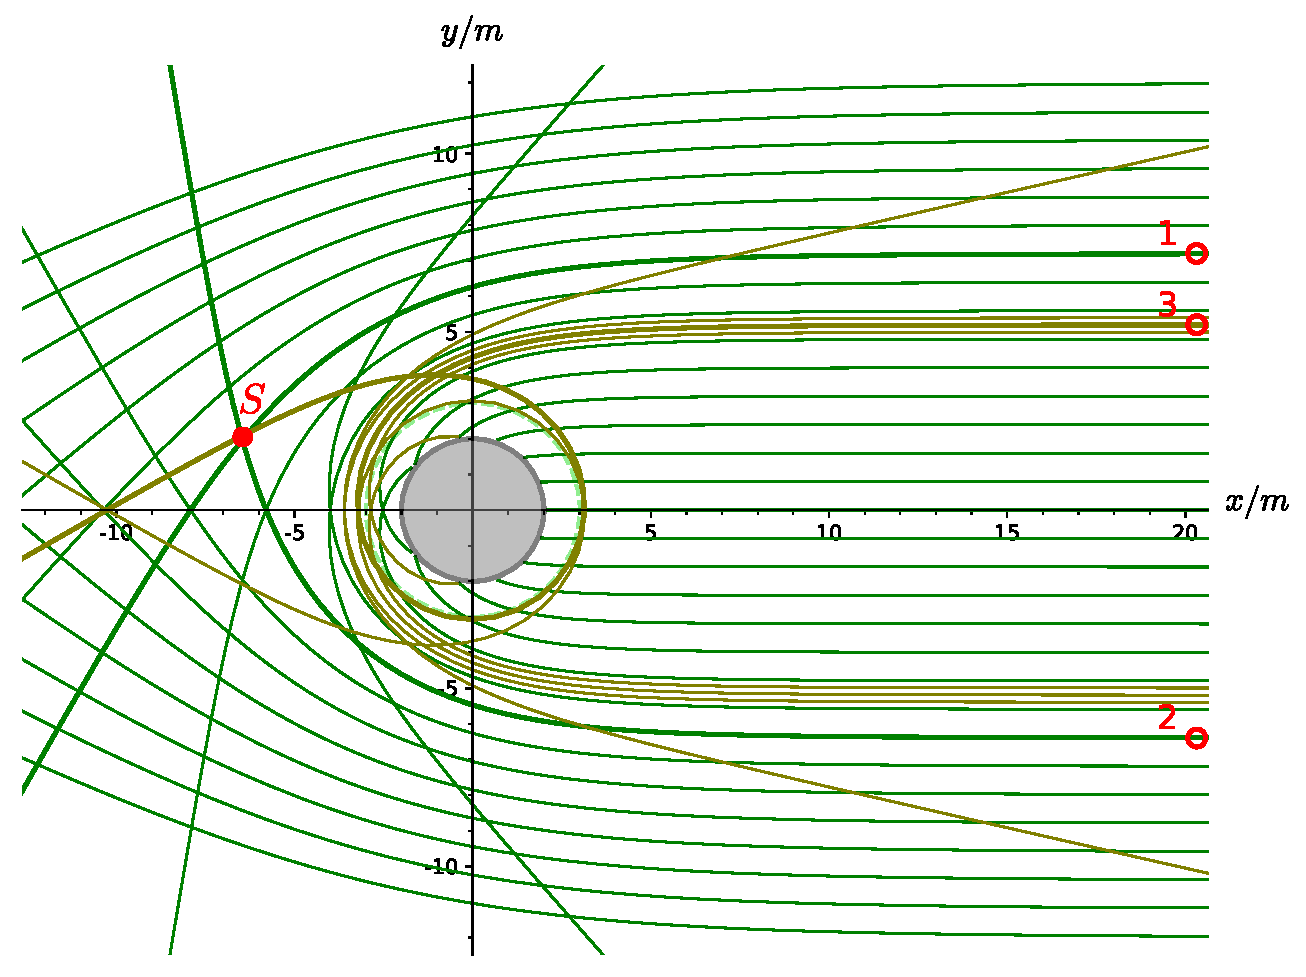
\includegraphics[width=0.9\textwidth]{ges_mult_images.pdf}}
\caption[]{\label{f:gis:mult_images} \footnotesize
Null geodesics in Schwarzschild spacetime with $\ph_\infty=0$ and various values of the impact parameter $b$.
The green ones have $b$ ranging from $-12 m$ to $12 m$, by steps of
$0.8 m$, while the olive ones have $b$ close to $b_{\rm c}$,
namely $b/m\in\{-5.4,-5.2,-5.0\} \cup \{5.0, 5.2, 5.4\}$. $S$ is a luminous point source
and three of its images for an observer at $y=0$ and $x\to + \infty$ are obtained by
following the drawn null geodesics through $S$.}
\end{figure}

To understand the formation of images on $\Obs$'s screen, a bunch of null
geodesics with $\ph_\infty=0$ is drawn in Fig.~\ref{f:gis:mult_images}.
$\Obs$ is located in the far right of this figure and
all the drawn geodesics eventually hit $\Obs$'s screen. Let us consider a luminous point source
$S$ in the surroundings of the black hole. From the drawing of Fig.~\ref{f:gis:mult_images},
three null geodesics of the $\ph_\infty=0$ family goes through $S$. They give rise to
three distinct images of $S$ on $\Obs$'s screen, which are represented by the
open circles labelled 1 to 3 in the right part of the figure. These three
geodesics can be distinguished by their deflection angle $\Theta$
and their winding number $n$ (cf. Sec.~\ref{s:gis:deflect_winding}).
The one giving image 1 is the less deflected: it has $\Theta \simeq - \pi/4$
and $n=0$, while that
of image 2 has $\Theta\simeq 2\pi/3$ and $n=0$.
The geodesic giving image 3 is much more deflected
it makes a full turn around
the black hole before reaching $\Obs$; it's winding number is $n=-1$ and
it has $\Theta\simeq -\pi/6$.
We note that the more deflected the geodesic,
the closer the image with respect to the circle $b = b_{\rm c}$ on $\Obs$'s
screen.

For the sake of clarity, only three images of the source $S$ have been
depicted in Fig.~\ref{f:gis:mult_images}, but there is actually an infinite
number of them: two per value of $|n|$ (the number of turns around the black hole)
--- one with $L>0$ and one with $L<0$. The selected geodesics in
Fig.~\ref{f:gis:mult_images} have $n=0$ and $L<0$ (image 1), $n=0$ and $L>0$
(image 2) and $n=-1$ and $L<0$ (image 3). The higher $|n|$, the closer the image
lies to the circle $b=b_{\rm c}$ on $\Obs$'s screen. Indeed, according to the
law (\ref{e:ges:b_bc_exp_Theta}), geodesics that perform $|n|$ turns around the
black hole have an impact parameter exponentially close to $b_{\rm c}$,
by a factor $\mathrm{e}^{- 2\pi |n|}$ (see also Fig.~\ref{f:gis:null_b2}).
Note that $\mathrm{e}^{- 2\pi}\simeq 1.9\times 10^{-3}$, so that any extra cycle
around the blak hole corresponds to a value of $b$ closer to $b_{\rm c}$
by two orders of magnitude.


If $S$, $\Obs$ and the black hole are not aligned, i.e. if $S$ is not located
on the $x$-axis, all the images of $S$ are aligned on $\Obs$'s screen: they
all lie in the plane defined by $S$, $\Obs$ and the black hole (plane of
Fig.~\ref{f:gis:mult_images}). This is a direct consequence of the spherical
symmetry of Schwarzschild spacetime.

In Fig.~\ref{f:gis:mult_images}, the source $S$ is rather close to the
black hole but it is worth to stress that
the multiple character of the images of a given
source is not due to the proximity between the source and the black hole.
Multiple images are formed for any source, even very far ones.
For instance, the source can lie \emph{behind} the
observer, i.e. one can have $x_S > x_{\Obs}$. This is clear if we consider
the lower-right panel of Fig.~\ref{f:gis:null_b1} (case $b=5.355\, m$):
a source with $x_S > x_{\Obs} \gg m$ and $y=5.355\, m$ gives an image on
$\Obs$'s screen at $b=5.355\, m$.

The reader may be puzzled by the compatibility between an infinite number
of images from a single source and the conservation of energy. There is
actually no issue here because one can show that the images are
fainter as $n$ increases. So in practice, only a few images would be visible.

\subsubsection{Link between the emission angle and the impact parameter}

In the above discussion, we have parametrized the null geodesics arriving
on the observer's screen by the impact parameter $b$. Let us relate the latter
to the emission angle in the source frame. To this aim, we consider that
the point source $S$, as depicted in Fig.~\ref{f:gis:mult_images}, is actually
the trace in the plane of the figure of the worldline of a static observer equipped
with a source of light, who we shall call the \emph{emitter} and denote
by $\Obs_{\rm em}$. Furthermore, we suppose that the rest frame of $\Obs_{\rm em}$
is an orthonormal tetrad
$\left(\w{u}_{\rm em}, \w{e}_{(r)}, \w{e}_{(\th)}, \w{e}_{(\ph)}\right)$ such
that the first spacelike vector, $\w{e}_{(r)}$, is always pointing towards the
black hole. More precisely, we set
\begin{subequations}
\label{e:gis:bo_Obs_em}
\begin{align}
& \w{u}_{\rm em} = \left( 1 - \frac{2m}{r_S} \right)^{-1/2} \wpar_t \\
& \w{e}_{(r)} = - \left( 1 - \frac{2m}{r_S} \right)^{1/2} \wpar_r \\
& \w{e}_{(\th)} = - r_S^{-1} \wpar_\th \\
& \w{e}_{(\ph)} = - r_S^{-1} \wpar_\ph ,
\end{align}
\end{subequations}
where $(\wpar_t, \wpar_r, \wpar_\th, \wpar_\ph)$ is the natural basis associated
with Schwarzschild-Droste coordinates and $r_S$ is the $r$-coordinate of
$S$, and hence of $\Obs_{\rm em}$.
It is immediate that $\left(\w{u}_{\rm em}, \w{e}_{(r)}, \w{e}_{(\th)}, \w{e}_{(\ph)}\right)$
is an orthonormal tetrad with respect to the Schwarzschild metric
(\ref{e:sch:Schwarz_metric_SD}). Moreover,
having a 4-velocity $\w{u}_{\rm em}$ collinear to the Killing vector $\wpar_t$
makes the observer $\Obs_{\rm em}$ static [cf. Eq.~(\ref{e:ges:u_Obs_xi})].

The 4-momentum $\w{p}$ of a photon emitted by $\Obs_{\rm em}$ in the equatorial
plane is given by Eqs.~(\ref{e:ges:comp_4_momentum}) and
(\ref{e:ges:dot_t_null})-(\ref{e:ges:dot_r_square_null}):
\be
    \w{p} = E \left( 1 - \frac{2m}{r} \right)^{-1} \wpar_t
        \pm E \sqrt{ 1 - b^2 U(r) } \, \wpar_r
        + \epsilon_L E \frac{b}{r^2} \, \wpar_\ph ,
\ee
where we have used Eq.~(\ref{e:ges:eff_pot_null}) to let appear $U(r)$
and Eq.~(\ref{e:ges:def_b}) to express $L$ in terms of $E$ and $b$.
Taking the value of $\w{p}$ at the emission point $S$ and using (\ref{e:gis:bo_Obs_em})
to express $\wpar_t$, $\wpar_r$ and $\wpar_\ph$ in terms of
$\Obs_{\rm em}$'s orthonormal tetrad, we get
\be \label{e:gis:p_eps_u_em_n}
    \w{p} = \veps_{\rm em} \left( \w{u}_{\rm em} + \w{n} \right) ,
\ee
where
\be
    \veps_{\rm em} := - \w{u}_{\rm em} \cdot \w{p} =
        E \left( 1 - \frac{2m}{r_S} \right)^{-1/2}
\ee
is the energy of the photon as measured by $\Obs_{\rm em}$ (cf. Sec.~\ref{s:fra:measure})
and
\be \label{e:gis:n_b_U_rS}
    \w{n} := \pm \sqrt{1 - b^2 U(r_S)} \, \w{e}_{(r)}
    - \epsilon_L b \sqrt{U(r_S)}\, \w{e}_{(\ph)}
\ee
is a unit spacelike vector orthogonal to $\w{u}_{\rm em}$:
$\w{n}\cdot\w{n} = 1$ and $\w{u}_{\rm em}\cdot\w{n} = 0$.
In view of (\ref{e:gis:p_eps_u_em_n}) and $\w{u}_{\rm em}\cdot\w{n} = 0$,
the linear momentum of the photon as measured by $\Obs_{\rm em}$ is
$\w{P} = \veps_{\rm em} \w{n}$ [cf. Eq.~(\ref{e:fra:p_E_P})].
We conclude that the unit vector $\w{n}$ gives the direction of emission
of the photon in $\Obs_{\rm em}$'s rest frame. Let us then define the \defin{emission
angle}\index{emission!angle} $\eta$ by
\be
    \w{n} = \cos\eta\, \w{e}_{(r)} + \sin\eta \, \w{e}_{(\ph)} .
\ee
Equation~(\ref{e:gis:n_b_U_rS}) yields immediately
\be \label{e:gis:cos_sin_eta_b}
 \cos\eta = \pm \sqrt{1 - b^2 U(r_S)} \qquad\mbox{and}\qquad
 \sin\eta = - \epsilon_L b \sqrt{U(r_S)} ,
\ee
from which we can express the impact parameter $b$ and
in terms of the emission angle $\eta$:
\be
    \encadre{ b = -\epsilon_L \frac{\sin\eta}{\sqrt{U(r_S)}} }.
\ee
\begin{remark}
Equation~(\ref{e:gis:cos_sin_eta_b}) is well posed because
$U(r)\geq 0$ for $r>2m$ [cf. Eq.~(\ref{e:ges:eff_pot_null})]
and the equation
of motion (\ref{e:ges:dot_r_square_null_b}) implies $b^{-2} - U(r_S) \geq 0$,
from which we get $0 \leq b^2 U(r_S) \leq 1$.
\end{remark}

\begin{figure}
\centerline{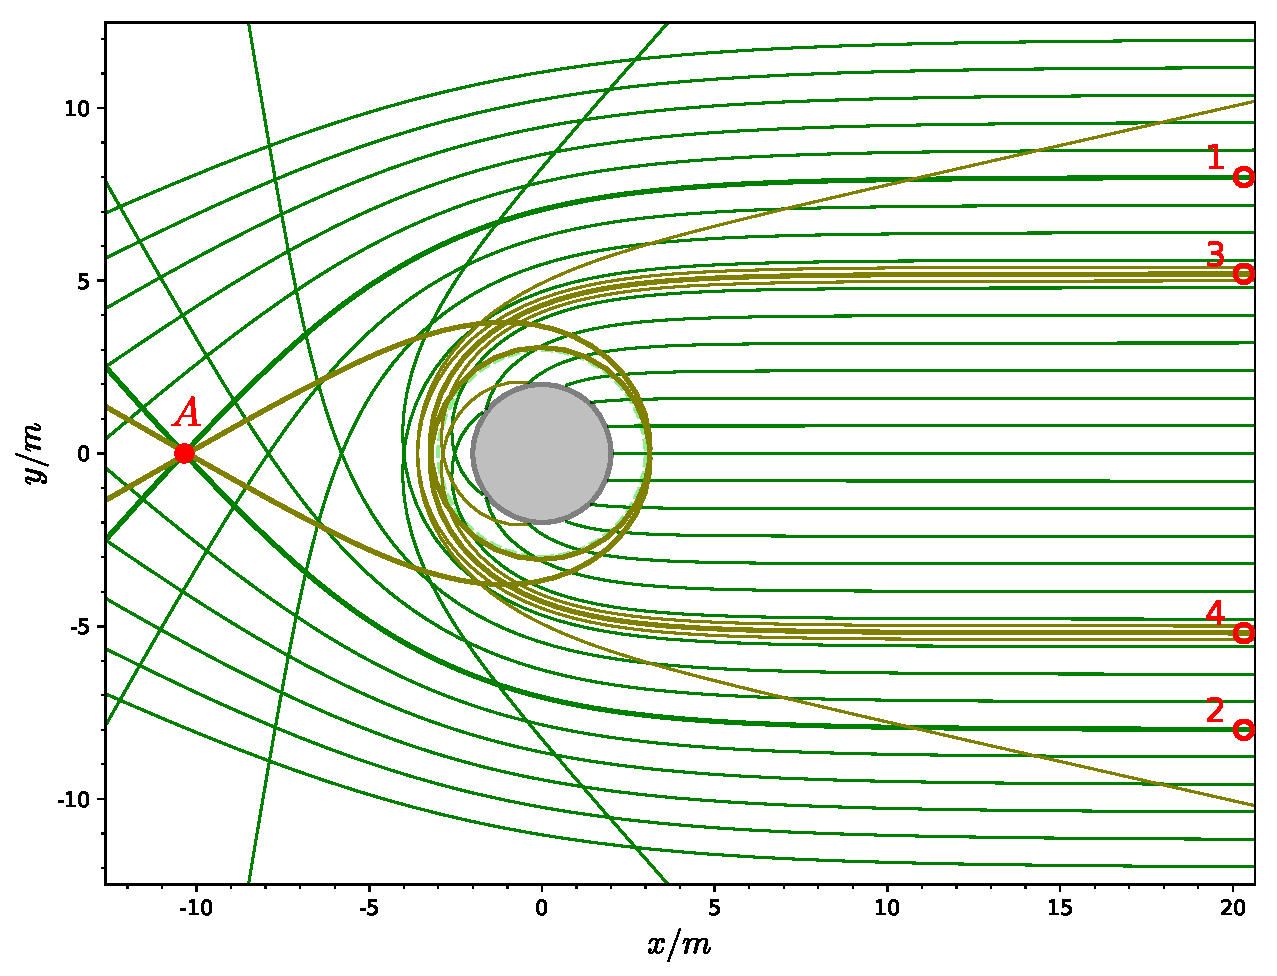
\includegraphics[width=0.9\textwidth]{ges_images_aligned.pdf}}
\caption[]{\label{f:gis:images_aligned} \footnotesize
Same as Fig.~\ref{f:gis:mult_images} but underlining four null geodesics
from a point source $A$ located on the $x$-axis, i.e.
aligned with the black hole and the observer.}
\end{figure}


\subsection{Aligned source and Einstein rings}

In the special case where the source is located on the $x$-axis, the images form
a series of concentric circles accumulating from above on the circle
$b = b_{\rm c}$. This is illustrated by the source $A$ in
Fig.~\ref{f:gis:images_aligned}. Four geodesics through the source are drawn,
given birth to four images that
are symmetric with respect to the $x$-axis, labelled 1, 3 and 2, 4 respectively.
Since in this case the plane of the figure is not privileged (one cannot speak
about the plane defined by $A$, $\Obs$ and the black hole, since they are aligned);
we deduce by rotation about the $x$-axis that $A$ generates images all along
circles centered on the origin in $\Obs$'s screen. Images 1 and 2 in Fig.~\ref{f:gis:images_aligned}
lie actually on the same circle, as well as images 3 and 4.
As for the non-aligned case, Fig.~\ref{f:gis:images_aligned} shows only a limited number of
images, but there is actually an infinite number of such images: the full image
of $A$ on $\Obs$'s screen is composed by a infinite sequence $(\mathscr{C}_n)_{n\in\mathbb{N}}$
of concentric circles
that accumulate exponentially fast onto the circle of radius $b = b_{\rm c}$.
Each circle $\mathscr{C}_n$ has a radius $b_n$ that is given approximately
by Eq.~(\ref{e:ges:b_bc_exp_Theta}), where $\Theta = \Theta_n$ is a function of
the position $x_A$ of $A$ on the $x$-axis. In particular $\Theta_n\to 0$
when $x_A\to -\infty$.
The outermost circle, $\mathscr{C}_0$, is called the
\defin{Einstein ring of}\index{Einstein!ring}\index{ring!Einstein --} $A$.
It is the only significant ring in astronomical images involving \emph{gravitational
lensing}\index{gravitational!lensing} by a massive foreground source (not necessarily
a black hole), which are in the context $|x_A|\gg m$ and $b\gg m$.
We may call $\mathscr{C}_n$ the $\bm{n^{\rm th}}$\defin{~Einstein ring of} $A$.
For $n\geq 1$, $\mathscr{C}_n$ is also called a \defin{relativistic Einstein ring of}
$A$. Indeed, these rings exist only in the case of a very relativistic central object, so that
photons can wind around it. On the contrary $\mathscr{C}_0$ exists even for non-relativistic
objects. In particular, in astronomical observations of Einstein rings performed up
to now, the central deflecting object is a galaxy or a galaxy cluster,
both being highly non-relativistic (very low compactness).

\subsection{Black hole shadow}

Let us determine the image on observer $\Obs$'s screen
when all the sources of light are very far, both
from the black hole and from $\Obs$. We may think of many stars
shining on the celestial sphere. To simplify the problem, we shall assume
that the black hole and the observer are surrounded by a distant
sphere $\mathscr{S}$ that is uniformly bright. In such a setting,
all values of $b > b_{\rm c}$ on $\Obs$'s screen, whatever the polar angle $\alpha$,
correspond to a null geodesic that originates from the shining sphere $\mathscr{S}$, while
this is not possible for $b \leq b_{\rm c}$.
This is clear on Fig.~\ref{f:gis:mult_images}: when traced backward from the right
($\Obs$ position), (i) null geodesics with $b > b_{\rm c}$ eventually end
up far away from the black hole, i.e. necessarily on $\mathscr{S}$, (ii) null geodesics
with $b < b_{\rm c}$ end up infinitely close to the black hole horizon
and (iii) null geodesics with $b = b_{\rm c}$ roll up indefinitely around
the photon sphere (cf. Figs.~\ref{f:gis:null_b_crit_from_inf_L_pos} and
\ref{f:gis:null_b_crit_from_inf_L_neg}).

The same conclusion can be reached
by considering the effective potential diagram in Fig.~\ref{f:gis:eff_pot_null}.
For concreteness, imagine that $\Obs$ is located at $r=15 m$ and that
the shining sphere $\mathscr{S}$ has a coordinate radius $r=20 m$.
These values allow us to put $\Obs$ and $\mathscr{S}$
in Fig.~\ref{f:gis:eff_pot_null} according
to our settings ($\mathscr{S}$ is encompassing both $\Obs$ and the black
hole), but one shall keep in mind that both $\Obs$ and $\mathscr{S}$
are assumed to lie at much larger values of $r$ (fulfilling $r\gg m$).
Only two kinds of geodesic
trajectories in Fig.~\ref{f:gis:eff_pot_null} diagram can reach $r = 15m$ ($\Obs$'s screen) with increasing values
of $r$ (the direction of observation): those of type 1 and those of type 3.
The latter ones originate necessarily from a region between the black hole
horizon and $\Obs$'s location, i.e. a region that does not intersect $\mathscr{S}$.
On the contrary, all the geodesics of type 1 must have had $r = 20 m$
in their past history, i.e. we may consider that they all have been emitted
by $\mathscr{S}$ inwards and have bounced on the potential barrier before
reaching $\Obs$'s screen in their outward motion.

So, both reasonings, that based on Fig.~\ref{f:gis:mult_images} and that
based on Fig.~\ref{f:gis:eff_pot_null}, led us to conclude that
\begin{greybox}
For a distant observer, the image of a uniformly bright sphere $\mathscr{S}$ surrounding
the black hole and the observer is a bright area fulfilling
the observer's screen, except for a central black disk of radius $b=b_{\rm c}$.
The latter is called the
\defin{black hole shadow}\index{black hole!shadow}\index{shadow!black hole --}.
\end{greybox}

\subsection{Image of an accretion structure}


\begin{hist}
Droste \cite{Drost1917}, Flamm \cite{Flamm1916}, Hilbert \cite{Hilbe1917a,Hilbe1917b}, Hagihara,  Darwin \cite{Darwi59} (multiple images of a point source, with accumulation just outside the critical radius), Synge \cite{Synge66}, Bardeen \cite{Barde73}, Luminet \cite{Lumin79,Lumin19}, Marck \cite{Marck96}

\end{hist}





